% Modified for use with JCC - Madhusudan Singh Copyright (C) (2012). All rights reserved.
%\documentclass[aip,reprint]{revtex4-1}
\documentclass[aip]{revtex4-1}

\setlength{\oddsidemargin}{0in}  %left margin position, reference is one inch
\setlength{\textwidth}{6.5in}    %width of text=8.5-1in-1in for margin
\setlength{\topmargin}{-0.5in}    %reference is at 1.5in, -.5in gives a start of about 1in from top
\setlength{\textheight}{9in}     %length of text=11in-1in-1in (top and bot. marg.) 
%\newenvironment{wileykeywords}{\textsf{Keywords:}\hspace{\stretch{1}}}{\hspace{\stretch{1}}\rule{1ex}{1ex}}

\usepackage{amsmath,amssymb}
\usepackage{graphicx}% Include figure files
%\usepackage{caption}
\usepackage{color}% Include colors for document elements
\usepackage{dcolumn}% Align table columns on decimal point
\usepackage{bm}% bold math
%\usepackage[numbers,super,comma,sort&compress]{natbib}
%\usepackage[nolists, nomarkers, figuresfirst]{endfloat}

\definecolor{background-color}{gray}{0.98}
\graphicspath{{data/}{images/}}

\begin{document}

%\title{Atomic pseudo-potentials for sp$^2$ carbon atoms}
\title{Atomic pseudo-potentials for reproducing the valence electron behaviour of sp$^2$ carbon atoms}
\author{Alexander Punter}
\author{Paola Nava}
\author{Yannick Carissan}
\affiliation{Aix Marseille Univ, CNRS, Centrale Marseille, iSm2, Marseille, France}

\begin{abstract}
A pseudo-potential system for recreating an sp\(^{2}\) carbon atom is built 
and tested as a building block for various pseudo-hydrocarbon chain and ring systems.  
This pseudo-system has a central charge of 1, thus it contains only one
electron. It is employed in \textsl{ab-initio} calculations in which several physical characterstics
including first ionisation and excitation energies, as well as the HOMO energy, 
are found to be well-reproduced by the pseudo-system.
\end{abstract}
\maketitle
%\begin{wileykeywords}
%Anisotropy, Pseudo-potential, $\pi$ system, Quantum Chemistry, Spin %contamination
%\end{wileykeywords}

\clearpage

%*****************Graphical Table of Contents******************** THIS IS MANDATORY *******************


\begin{figure}[h]
\centering
\colorbox{background-color}{
\fbox{
\begin{minipage}{1.0\textwidth}
%\includegraphics[width=50mm,height=50mm]{cc.eps} % Pick only one of the two styles by uncommenting the corresponding \includegraphics
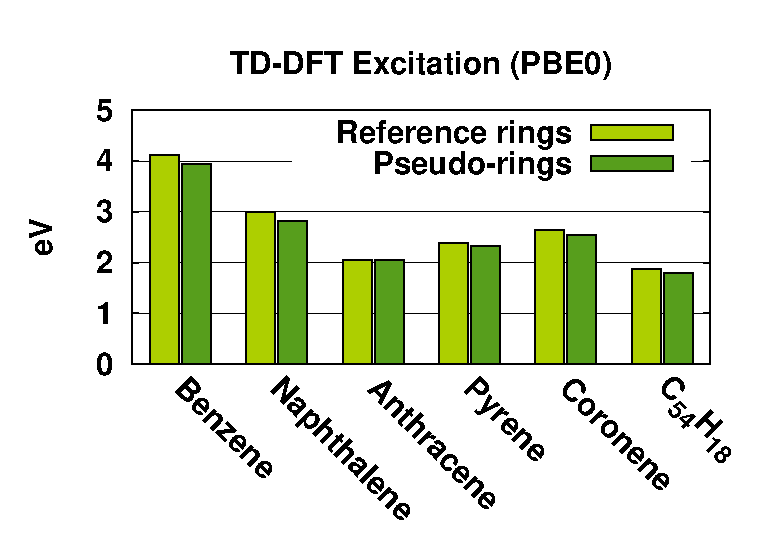
\includegraphics[width=50mm,height=50mm]{ring_pbe0_tddft}
%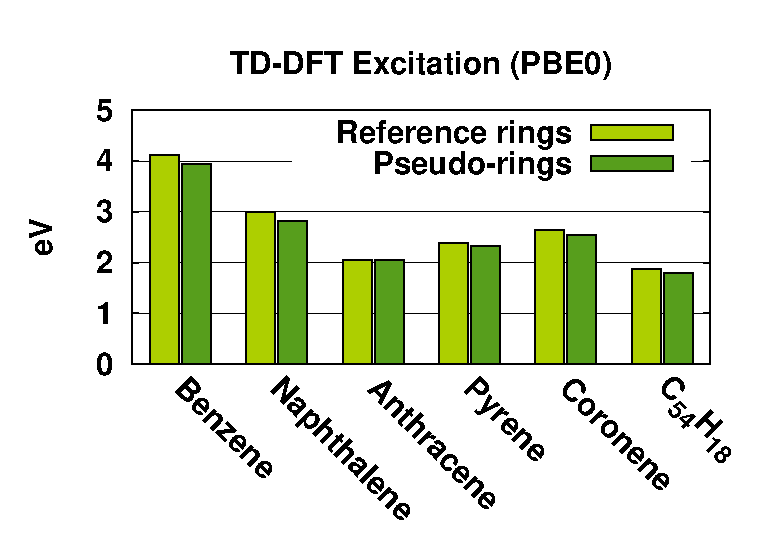
\includegraphics[width=110mm,height=20mm]{ring_pbe0_tddft}
\\
A pseudo-potential system for recreating an sp\(^{2}\) carbon atom is built
and tested as a building block for various pseudo-hydrocarbon chain and ring systems.
This pseudo-system has a central charge of 1, thus it contains only one
electron. It is employed in \textsl{ab-initio} calculations in which several physical characterstics
including 1\textsuperscript{st} ionisation and excitation energies, as well as the HOMO energy,
are found to be well-reproduced by the pseudo-system.
\end{minipage}
}}
\end{figure}

% makes references listed with 1., 2., etc.  
  \makeatletter
  \renewcommand\@biblabel[1]{#1.}
  \makeatother

\bibliographystyle{apsrev}

\renewcommand{\baselinestretch}{1.5}
\normalsize


\clearpage
% 

\section{Introduction}
\newcounter{customItem}
\newcommand{\showCustomItem}{\refstepcounter{customItem}\roman{customItem}}

%For most of the quantum chemistry calculations, the system can be divided into two parts:
%the active part, \emph{i.e.} the part of the molecule one is interested in and
%the inactive part, which is to be taken into account in order to fulfill chemical requirements.
It is a common idea that a chemical system can be thought of as comprised of
two parts:
an active one, where most of the chemistry takes place, and an inactive
one, which must be taken into account in order to fulfill chemical requirements.
Based on this general statement, many successful theoretical approaches have been developed.
Among them can be cited QM/QM' or QM/MM methods (\showCustomItem), where 
the active region that usually contains several atoms is
treated at a high level of calculation, while the inactive part is treated at a 
lower level of theory.\cite{chung_oniom_2015}
Fragmentation methods split the complete problem into smaller parts and combine individual calculations
on these fragments to recover the properties of the overall system.\cite{gordon_effective_2001,steinmann_effective_2012}
Frozen density embedding techniques (\showCustomItem) replace part of a molecule, or 
its surroundings,
by a frozen electronic density extracted on a reference system.\cite{wesolowski_frozen-density_2015}
They are an extension of the frozen core approximation, already used to reduce
the number of parameters to be optimised in the self consistent field calculation.
In the framework of this work, the pioneering work of Rivail \emph{et al.} must be mentionned:
the total wave function is optimized with some molecular orbitals kept frozen.\cite{ASSFELD1996100}

In this article we shall focus on pseudo-potential techniques, which also
divide the chemical problem into two parts.
Effective core potentials (\showCustomItem) are commonly employed for atoms: 
core electrons (and effects due to the corresponding nuclear charge) are
replaced by an operator fast to evaluate and the active electrons are treated
explicitly.\cite{dolg_relativistic_2012}
In the same vein, model potentials (\showCustomItem) replace a frozen electronic density (computed from the atom)
by some operators, the number of which depends on the level of
refinement required.\cite{huzinaga_1994_1995}

The effective group potentials (\showCustomItem) bridge the frozen density and the core potential
approaches: using core potential extraction techniques, effects due to the implicit 
electron density (and corresponding nuclear charge) 
are reproduced by a mono-electronic operator.\cite{carissan_what_2006, raynaud_multicentered_2010}
However, while effective core potentials and model potentials intend to 
reproduce atomic properties,
effective group potentials aim at mimicking the effect of atoms involved in one or more chemical
bonds. The cyclopentadienyl group has, for instance, been successfully extracted.\cite{carissan_what_2006}
In this example, the active part consisted of six electrons (the $\pi$ electrons) and six
nuclear charges, with the pseudo-potential replacing all the rest, including the hydrogen atoms.
Even if the $\sigma / \pi$ separability suggested how to define the active and the inactive parts,
carbon atoms are hybridized and the core/valence distinction is not 
strictly defined.

The theoretical background to extract effective group pseudo-potentials  can be traced back 
to several contributions in the 80's and  90's.\cite{Nicolas1980a, huzinaga_effective_1991, huzinaga_1994_1995, EGP5, EGP6, EGP9}
In 1992 Katsuki built molecular potentials based on Huzinaga's model potentials.\cite{katsuki_molecular_1992,katsuki_spectral_1993}
 In his work on this subject, Huzinaga emphasises that pseudo-potentials should maintain three effects of the
'dormant' electrons on the active ones: the Coulomb, the exchange and the 'no-collapse' term.\cite{huzinaga_effective_1991}
Following his proposal, for an atom where active and dormant electrons have been separated, the Hamiltonian reads:
\begin{equation}
\label{eq:atomicHamiltonian}
\hat{H} = \sum_{i=1}^n \hat{h}(i) +\sum_{i<j}\frac{1}{r_{ij}}
\end{equation}
with $\frac{1}{r_{ij}}$ the bi-electronic interaction
between explicitly treated active electrons and
the mono-electronic operator:
\begin{equation}
\label{eq:monoElectronicOperator}
\hat{h}(i) = -\frac{1}{2}\Delta_i - \frac{(Z-Z_c)}{r_i}+\hat{V}(i) + \hat{\sigma}(i)
\end{equation}
where $\Delta_i$ is the Laplacian of the coordinates of electron $i$, and 
$Z_C$ is the number of core electrons withdrawn from the reference system.
The operator $\hat{\sigma}(i)$ is the 'no-collapse' term that prevents active electrons
collapsing into the dormant region. The operator $\hat{V}(i)$ reproduces the 
Coulomb and exchange interactions:
\begin{equation}
\label{eq:HuzinagaMPVersion1Potential}
\hat{V} = \frac{1}{r}\left[\sum_IA_I\exp(-\alpha_I r^2)+\sum_JB_Jr\exp(-\beta_J r^2)\right]
\end{equation}

To take into account the fact that dormant electrons are removed from the
system, the nuclear charge is modified by the $Z_c$ value.
Yet, as the effective charge felt by the active electrons is likely not to be an integer,
the modification of the value of the nuclear charge is scaled in $\hat{V}$.
In this operator we notice that the \(r^{-1}\) behavior is mantained for the first term 
(the Coulomb one).

%Let us follow Huzinaga in his enlightening work.\cite{huzinaga_effective_1991}
%In order to extract a meaningful potential, he states that for electron/electron interactions, 
%"the most important effect is that the exclusion principle prevents active electrons
%from collapsing into the dormant region.
%The second is the exchange energy terms between the dormant and active electrons
%through their electrostatic interaction."
%For an atom, the Hamiltonian reads:
%\begin{equation}
%\label{eq:atomicHamiltonian}
%\hat{H} = \sum_{i=1}^n \hat{h}(i) +\sum_{i<j}\frac{1}{r_{ij}}
%\end{equation}
%with $\frac{1}{r_{ij}}$ the bi-electronic interaction
%between explicitly treated active electrons and
%the mono electronic operator:
%\begin{equation}
%\label{eq:monoElectronicOperator}
%\hat{h}(i) = -\frac{1}{2}\Delta_i - \frac{(Z-Z_c)}{r_i}+\hat{V}(i) + \hat{\sigma}(i)
%\end{equation}
%where
%$\Delta_i$ is the laplacian of the coordinates of electron $i$,
%$Z_C$ is the number of core electrons withdrawn from the reference system,
%$\hat{V}(i)$ the pseudo-potential which reproduces the electrostatic
%interaction between the dormant and active electrons
%and $\hat{\sigma}(i)$ the operator, which models the exclusion principle
%and prevents active electrons from collapsing into the dormant region.
%To take into account the fact that dormant electrons are removed from the
%system, the nuclear charge is modified by the $Z_c$ value.
%Yet, as the effective charge felt by the active electrons is likely not to be an integer,
%the modification of the value of the nuclear charge is scaled in $\hat{V}$.
%Depending on the version used, this modification differs.
%In this work, we take as a reference version 1 as defined in
%Huzinaga's lecture\cite{huzinaga_1994_1995}:
%\begin{equation}
%\label{eq:HuzinagaMPVersion1Potential}
%\hat{V} = \frac{1}{r}\left[\sum_IA_I\exp(-\alpha r^2)+\sum_JB_Jr\exp(-\beta r^2)\right]
%\end{equation}
%In this model potential version, $\hat{\sigma}$ is defined as:
%\begin{equation}
%\label{eq:HuzinagaMPVersion1Sigma}
%\hat{\sigma} = -\sum f_c\epsilon_c\left|\phi_c\right>\left<\phi_c\right|
%\end{equation}
%with $\epsilon_c$ the eigenvalue of the core orbital $\phi_c$ and
%$f_c$ an optimised parameter.
%In the other versions of model potentials, $f_c=2$, as suggested earlier.\cite{houjer_aspects_1978}

%In the present work, we shall optimise the parameters in $\hat{V}$ and $\hat{\sigma}$
%for hybridised atoms.
%Before going further, it is important to stress that hybridisation implies that the
%$\left\{\phi_c\right\}_i$ are linear combination of atomic orbitals and that
%$\hat{V}$ should no more be spherical.
%This loss of isotropy combined with the loss of clear core/valence separation
%will imply constraints during the extraction process.

In the present work, the aim is 
to propose a methodology for extracting a potential for
a hybridised carbon atom (here an $sp^2$ carbon atom), which can then be
used as a building block for constructing chemical systems. This carbon atom
will contain explicitly one nuclear charge and one electron.
Moreover, the method should be usable 
%In this work, we aim at developing a method usable 
out of the box in any standard quantum chemistry software.
Thus, no modification of the source code should be done.
This supplementary constraint will be fulfilled by strategically positioning the pseudo-potentials
we intend to use. 

Pseudo-potentials for hybridised carbon
atoms have been already successfully extracted in a previous work of ours.\cite{drujon_pseudopotentials_2013}
There, our attention was focused on the 'no-collapse' term, and 
functions in the pseudo-potential shift up unwanted orbitals and correctly place the energy of the
wanted orbitals.
A drawback of this method was that some pseudo-potentials had to be put precisely at the center
of each bond.
Thus, those pseudo-potentials could not be considered as purely local as they were not defined solely
with respect to the position of the atom they applied to.
This previous work should therefore be regarded as a proof-of-concept.
In this new version, we include more physical meaning in our model, 
by placing pseudo-potentials that mimic Coulomb interactions among both the active and dormant electrons, and the shielded nuclear charge. 
The new pseudo-potentials are fully atomic: the position of the atom
determines completely where the potentials are placed in space in the best possible manner
when dealing with hybridised atoms (as hybridisation destroys isotropy, the preferred orientations
must be given to define the pseudo-potential).
Furthermore, the way we define the pseudo-potentials in the current work, do not require
the no-collapse term.

This article is structured as follows.
In the methodology part firstly gives the general definition of the pseudo-potential, which
we develop.
Secondly the particular case of the CH$_3^\bullet$ radical is detailed as it gives access
to some phisically grounded values.
In a third part, the optimal pseudo-potential is defined. Details of the step by step extraction
are given in the supplementary materials.
The application part focuses on the performances of the optimal pseudo-potential.
It is shown that the properties can be well reproduced except when dealing with
systems in which spin contamination is large.
For these cases, a solution is provided.

\section{Methodology}

\subsection{General pseudo-potential definition}

%As in our previous work\cite{drujon_pseudopotentials_2013},
%we take CH\(^{\bullet}_{3}\) as our starting system to be reproduced.
%It is the smallest system containing one and only one sp$^2$ hybridised carbon atom.
%This choice allows us to isolate the different electrostatic interactions
%to build a physically meaningful model.
We make use of two kinds of gaussian pseudo-potentials \cite{me_structure_theory}, of \(s\) and \(p\) shapes. As we want to avoid modifying the quantum chemistry software itself, the pseudo-potentials have a semi-local form.
The multi-centered pseudo-potentials that we build read as follows:
\begin{equation}
\label{eq:ourPP}
\hat{W} = \frac{1}{r}\left[%
\underbrace{\sum_IA_I\exp(-\alpha_I r^2)\left|Y_{1,m}\right>\sum_m\left<Y_{1,m}\right|}_{\text{p projectors}}%
+%
\underbrace{\sum_JC_Jr\exp(-\gamma_J (r-r^0_J)^2)\left|Y_{0,0}\right>\left<Y_{0,0}\right|}_{\text{s projectors}}%
\right]
\end{equation}
with $Y_{0,0}$ the $s$ spherical harmonic, $Y_{1,m}$ the $p$ spherical harmonics
and $r^0_J$ the relative fixed position of the $J^{th}$
potential with respect to the origin of the pseudo-atom, which carries the pseudo-potentials.
By analogy with Huzinaga model potentials defined in (\ref{eq:HuzinagaMPVersion1Potential})
we can say that the $p$ projectors aim to mimic a coulombic interaction,
while the $s$ potentials have the task of recovering part of the bi-electronic interaction
between the dormant and the active electrons.

As will be discussed in the following sections,
the \(p\) pseudo-potential allows to reproduce atomic properties, when the
\(s\)-potentials mimic electrostatic electron pair repulsion. The pseudo-potentials are mono-electronic operators, thus they shall not be able to reproduce fully bi-electronic interactions. Knowing this, we adjust the parameters of the \(s\)-potentials for the pseudo-system to have a wavefunction in which properties, such as spatial extent, energy and excitation energies, are as close as possible to those of the reference system.

\subsection{Extraction for the CH$_3^\bullet$ radical}
\label{section:potential_derivation}
As in our previous work\cite{drujon_pseudopotentials_2013},
we take CH\(^{\bullet}_{3}\) (d$_{CH}=2.0466 a.u.$) as our starting system to be reproduced.
It is the smallest system containing one and only one sp$^2$ hybridised carbon atom.
This choice allows us to isolate the different electrostatic interactions
to build a physically meaningful model.

\begin{figure}
\begin{center}
%\includegraphics[width=0.2\columnwidth,keepaspectratio=true]{cc.eps}
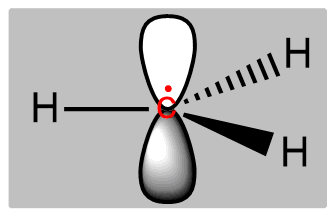
\includegraphics[width=8cm]{ch3.png}
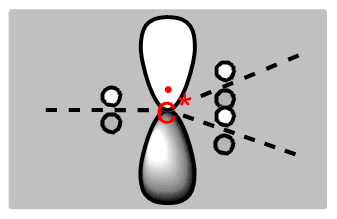
\includegraphics[width=8cm]{pseudoch3.png}
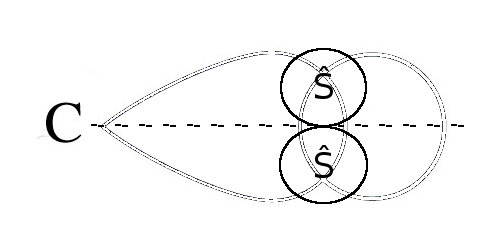
\includegraphics[width=8cm]{tm_sp2_potentials.png}
%\caption{Diagrams of CH\(^{\bullet}_{3}\) (left) and pseudo-CH\(^{\bullet}_{3}\) (right, below) molecules. The pseudo-CH\(^{\bullet}_{3}\) diagrams display the \(s\) and \(p\)-potential positions, and the distances \(d\) and \(c\).}
%\label{figure:ref_pseudo_diagram}
\end{center}
\caption{Diagrams of CH\(^{\bullet}_{3}\) (left) and pseudo-CH\(^{\bullet}_{3}\)
(right, below) molecules.
The pseudo-CH\(^{\bullet}_{3}\) diagrams display the \(s\) and \(p\)-potential positions,
and the distances \(d\) and \(c\).
In this article $d=2.0 a.u.$ and $c=0.25 a.u.$}
\label{figure:ref_pseudo_diagram}
\end{figure}

Figure \ref{figure:ref_pseudo_diagram} displays the final pseudo-system: the CH\(^{\bullet}_{3}\) radical has been replaced by
a hydrogen-like "pseudo-carbon", with a nuclear charge of \(Z_{nucleus} = 1\), and one electron occupying the \(p_{z}\) orbital. 
There are now no H atoms, and the system is surrounded by three potential sets at a planar distance of \(d\), each consisting of 
two \(s\)-shaped potentials with a distance above and below the \(xy\)-plane of \(c\). A further \(p\)-shaped potential is applied
directly to the pseudo-carbon.

This gives multiple variables we can use to manipulate the properties of the system.
We can alter the strength and diffuseness of the \(p\) and \(s\) potentials themselves,
as well as vary the distances \(d\) and \(c\) by moving the \(s\)-potentials.
In this article, we fix \(c = 0.25\;a.u.\).

%\subsection{Making Potentials Physically Meaningful}
%\label{section:potential_derivation}

It is possible to obtain the potential parameters entirely by empirical means, in principle. However, we can make a more informed guess at some starting parameters from which to optimise. Clearly the assumption that \(Z = 1\) is unrealistic. Slater's Rules\cite{slatersrules} suggest that, with the screening effect, the \(p_{z}\) electron of a carbon atom should experience a charge of \(Z = 2.4\). To mimic the effect of an electron-screened nucleus, we can use a \(p_{z}\) pseudo-potential. In order to make an educated guess of the parameters of this new potential, we need to find an expression for \(Z_{eff}(\langle r \rangle)\); \(Z_{eff}\) being the total nuclear attraction the electron would feel in the real CH\(^{\bullet}_{3}\) system, taking into account the screening effect of the core electrons that would be present in an all-electron model; and \( \langle r \rangle \) being the expected distance of the electron from the nucleus.
%	The generic forms of Gaussian Type Orbitals for \(s\) and \(p_{z}\) are [REF]
%\begin{equation}
%\psi_{s} = re^{-\alpha r^{2}},\qquad	\psi_{p_{z}} = r \cos \theta e^{-\alpha r^{2}}
%\end{equation}

The analytical form of the \(p_{z}\) orbital for a hydrogen-like atom is\cite{nyu_h_solutions}
\begin{equation}
\phi_{210} = \frac{1}{\sqrt{\pi}} \frac{Z_{eff}}{2a_{0}} ^{\frac{5}{2}} re^{-\frac{Z_{eff}r}{2a_{0}}} \cos \theta
\end{equation}
and from this we obtain 
\begin{equation}
\label{equation:PsirPsi}
\langle \phi_{210} | r | \phi_{210} \rangle = \frac{5a_{0}}{Z_{eff}}
\end{equation}
Next, we need to find a value for \( \langle r \rangle \). We can do this by calculating

\begin{equation}
\langle r \rangle = \langle \psi_{p_{z}} | r | \psi_{p_{z}} \rangle
\label{equation:exp_r}
\end{equation}

%%
%% \begin{equation}
%% \langle r \rangle = \lambda B \lambda^{T}
%% \label{equation:exp_r}
%% \end{equation}
%% where \(\lambda\) are the Symmetrised Atomic Orbital Shells taken from the molecular orbital files of a reference calculation of a CH\(^{\bullet}_{3}\) %% radical, and B is the matrix of \(\langle \psi_{p_{z}} | r | \psi_{p_{z}} \rangle\) values, appropriately normalised and contracted according to the basis %% set used (in this case, def-SV(P) \cite{defsvp}).
%%

 where \(\psi_{p_{z}}\) are the molecular orbitals extracted from a reference calculation of CH\(^{\bullet}_{3}\). From Equation \ref{equation:exp_r}, we have \( \langle r \rangle \approx 1.8\;a.u.\) and therefore we can see from Equation \ref{equation:PsirPsi} that \(Z_{eff} \approx 3.6\). Even if we shall use the semi-local pseudo-potential definition for the calculations, for a quick evaluation of overlap effects between the basis set and the pseudo-potential, we assume a non-local pseudo-potential definition. We define:
\begin{equation}
S = \langle \psi_{p_{z}} | \chi \rangle
\end{equation}
the overlap between a molecular orbital \(\psi_{p_{z}}\), and \(\chi\), taken from our non-local pseudo-potential definition \cite{huzinaga_effective_1991}
\begin{equation}
\chi = e^{-\alpha r^{2}},\qquad \widehat{p} = Z_{pseudo} | \chi \rangle \langle \chi |
\end{equation}
leading us to
\begin{equation}
\langle \widehat{Z} \rangle = \langle \psi_{p_{z}} | \widehat{Z} | \psi_{p_{z}} \rangle = \langle \psi_{p_{z}} | Z_{pseudo} | \chi \rangle \langle \chi | \psi_{p_{z}} \rangle = Z_{pseudo} S^{2}
\end{equation}
Finally, knowing that our hydrogen-like pseudo-system already contains a charge, \(Z_{nucleus}=1\), which we subtract from the desired \(Z_{eff}\) with whch we want to influence our \(p_{z}\) electron, leaving us with
\begin{equation}
Z_{pseudo} = (Z_{eff} - Z_{nucleus})S^{-2}
\end{equation}

We now have the power to choose a \(p_{z}\) pseudo-potential solely based on the Gaussian
exponent, and the \(Z_{eff}\) then follows from the above.
Clearly, the exponent should be chosen to give us a strong overlap with the molecular
orbital we wish to influence.
Hence we arrive at a \(p_{z}\)-potential that should be physically meaningful.
The maximum overlap possible ($\approx$ 0.79) was obtained with an exponent
of 0.295 a.u., which leads to a coefficient of -3.267 a.u.

\subsection{Extraction in the general case for C sp$^2$ atoms}
\label{section:csp2_extraction}
The CH$_3^\bullet$ radical allowed us to test our model but is not useful
when dealing with $\pi$ molecular interactions as it does not contain
any $\pi$ bond.
We intend to extract a pseudo-potential, which interacts properly with 
other $\pi$ carrying atoms, would they be pseudo-system or real systems.
Furthermore, we expect our hypothesis to be grounded and should be able to
extract parameters on as few data as possible.
Thus, we extracted the optimal pseudo-potential by a step by step procedure described in 
the supplementary materials on the smallest $\pi$ system: the ethylene molecule.
Based on Equation \ref{eq:ourPP}, we define the complete pseudo potential as:

\begin{equation}
\label{eq:ourPPwithparams}
\hat{W} = \frac{1}{r}\left[%
\sum_IA_I\exp(-\alpha_I r^2)\left|Y_{1,m}\right>\left<Y_{1,m}\right|+
\sum_JC_Jr\exp(-\gamma_J (r-r^0_J)^2)\left|Y_{0,0}\right>\left<Y_{0,0}\right|
\right]
\end{equation}

\begin{table}[ht]
\begin{tabular}{llll}
\hline\hline
$s$ potential & $C_J=1.5$ & $\gamma_J=0.5$   & $r^0_J=0.5590$\\
$p$ potential & $A_I=-3.91$ & $\alpha_I=0.624$ &  \\
\hline
\hline
\end{tabular}
\caption{\label{tab:params}Optimal parameters obtained for the pseudo 
$\pi$ carbon atom (values in atomic units) at the HF level of theory.}
\end{table}

With parameters defined in Table \ref{tab:params}, the potential reproduces the properties of the ethylene $\pi$ cloud system with a good accuracy: relative errors on the ionisation energy and the energies of the HOMO orbital of 8\% and 3\% respectively (Table \ref{tab:res_ourPP}).

\begin{table}[ht]
\begin{tabular}{llll}
\hline\hline
& $\Delta_{ST}$  & I.E.  & $\varepsilon_{HOMO}$  \\
\hline
Reference Values & -3.533 & -9.091 & -10.363 \\
Optimal pseudo-potential & -3.533 & -9.806 & -10.062 \\
\hline\hline
\end{tabular}
\caption{\label{tab:res_ourPP}Comparison of the
singlet-triplet splitting ($\Delta_{ST}$), ionisation
energy (I.E.) and energy of the HOMO orbital ($\varepsilon_{HOMO}$)
of the reference ethylene molecule
and its reproduction with the optimal pseudo potential obtained in this work.
The $\Delta_{ST}$ values were obtained as the difference
between the lowest triplet (in an unrestricted formalism) and the lowest singlet state
(in a restricted formalism).
Calculations are performed at the HF level, values are in atomic eV.}
\end{table}

\section{Results and discussion}

\subsection{Computational Details}

All Hartree-Fock (HF), Density Functional Theory (DFT) and Time-Dependent DFT (TD-DFT) calculations
are performed with TURBOMOLE 7.1 \cite{TURBOMOLE}.
The basis set used throughout is def-SV(P) \cite{defsvp}.
Wherever possible, planar (C\(_{S}\)) symmetry is used.
The convergence energy is \(10^{-7}\)H (\texttt{\$scfconv = 7}) for SCF and \(10^{-6}\)H for DFT.
When running these calculations the occupation of orbitals is specified manually in the TURBOMOLE control file.

\textbf{Chain Alkenes, Ring Molecules}. In additional to Hartree-Fock calculations, DFT is used with PBE0, PBE, TPSS and TPSSh functionals. \cite{pbe0,pbe,tpss,tpssh} The integration grid size is set at \(m4\). Also used are TD-DFT calculations, where the Tamm-Dancoff approximation (CIS) \cite{tammdancoff} is switched on to avoid triplet instability.

\subsection{Alkene chains: C\(\mathbf{_{2n}}\)H\(\mathbf{_{2n+2}}\), \(\mathbf{2 \leq n \leq 12}\)}

Taking these optimal parameters we test them against a series of chain alkenes up to length C\(_{12}\)H\(_{14}\), using a variety of functionals. In each case, the geometry of the reference system is optimised according to the method used, 
before taking the reference geometry and applying the pseudo-potentials from Table \ref{tab:res_ourPP}. 
Figure \ref{fig:alkenes_hf_dft} shows the results.
Table \ref{table:alkene_errors} gives a breakdown of the percentage errors for each method across all molecules tested. The pattern of increasing HOMO energy and decreasing cation-singlet and triplet-singlet energies seen in the reference systems is well replicated by the pseudo-alkenes, with the energies following the same gradient.

\begin{figure}
\begin{center}
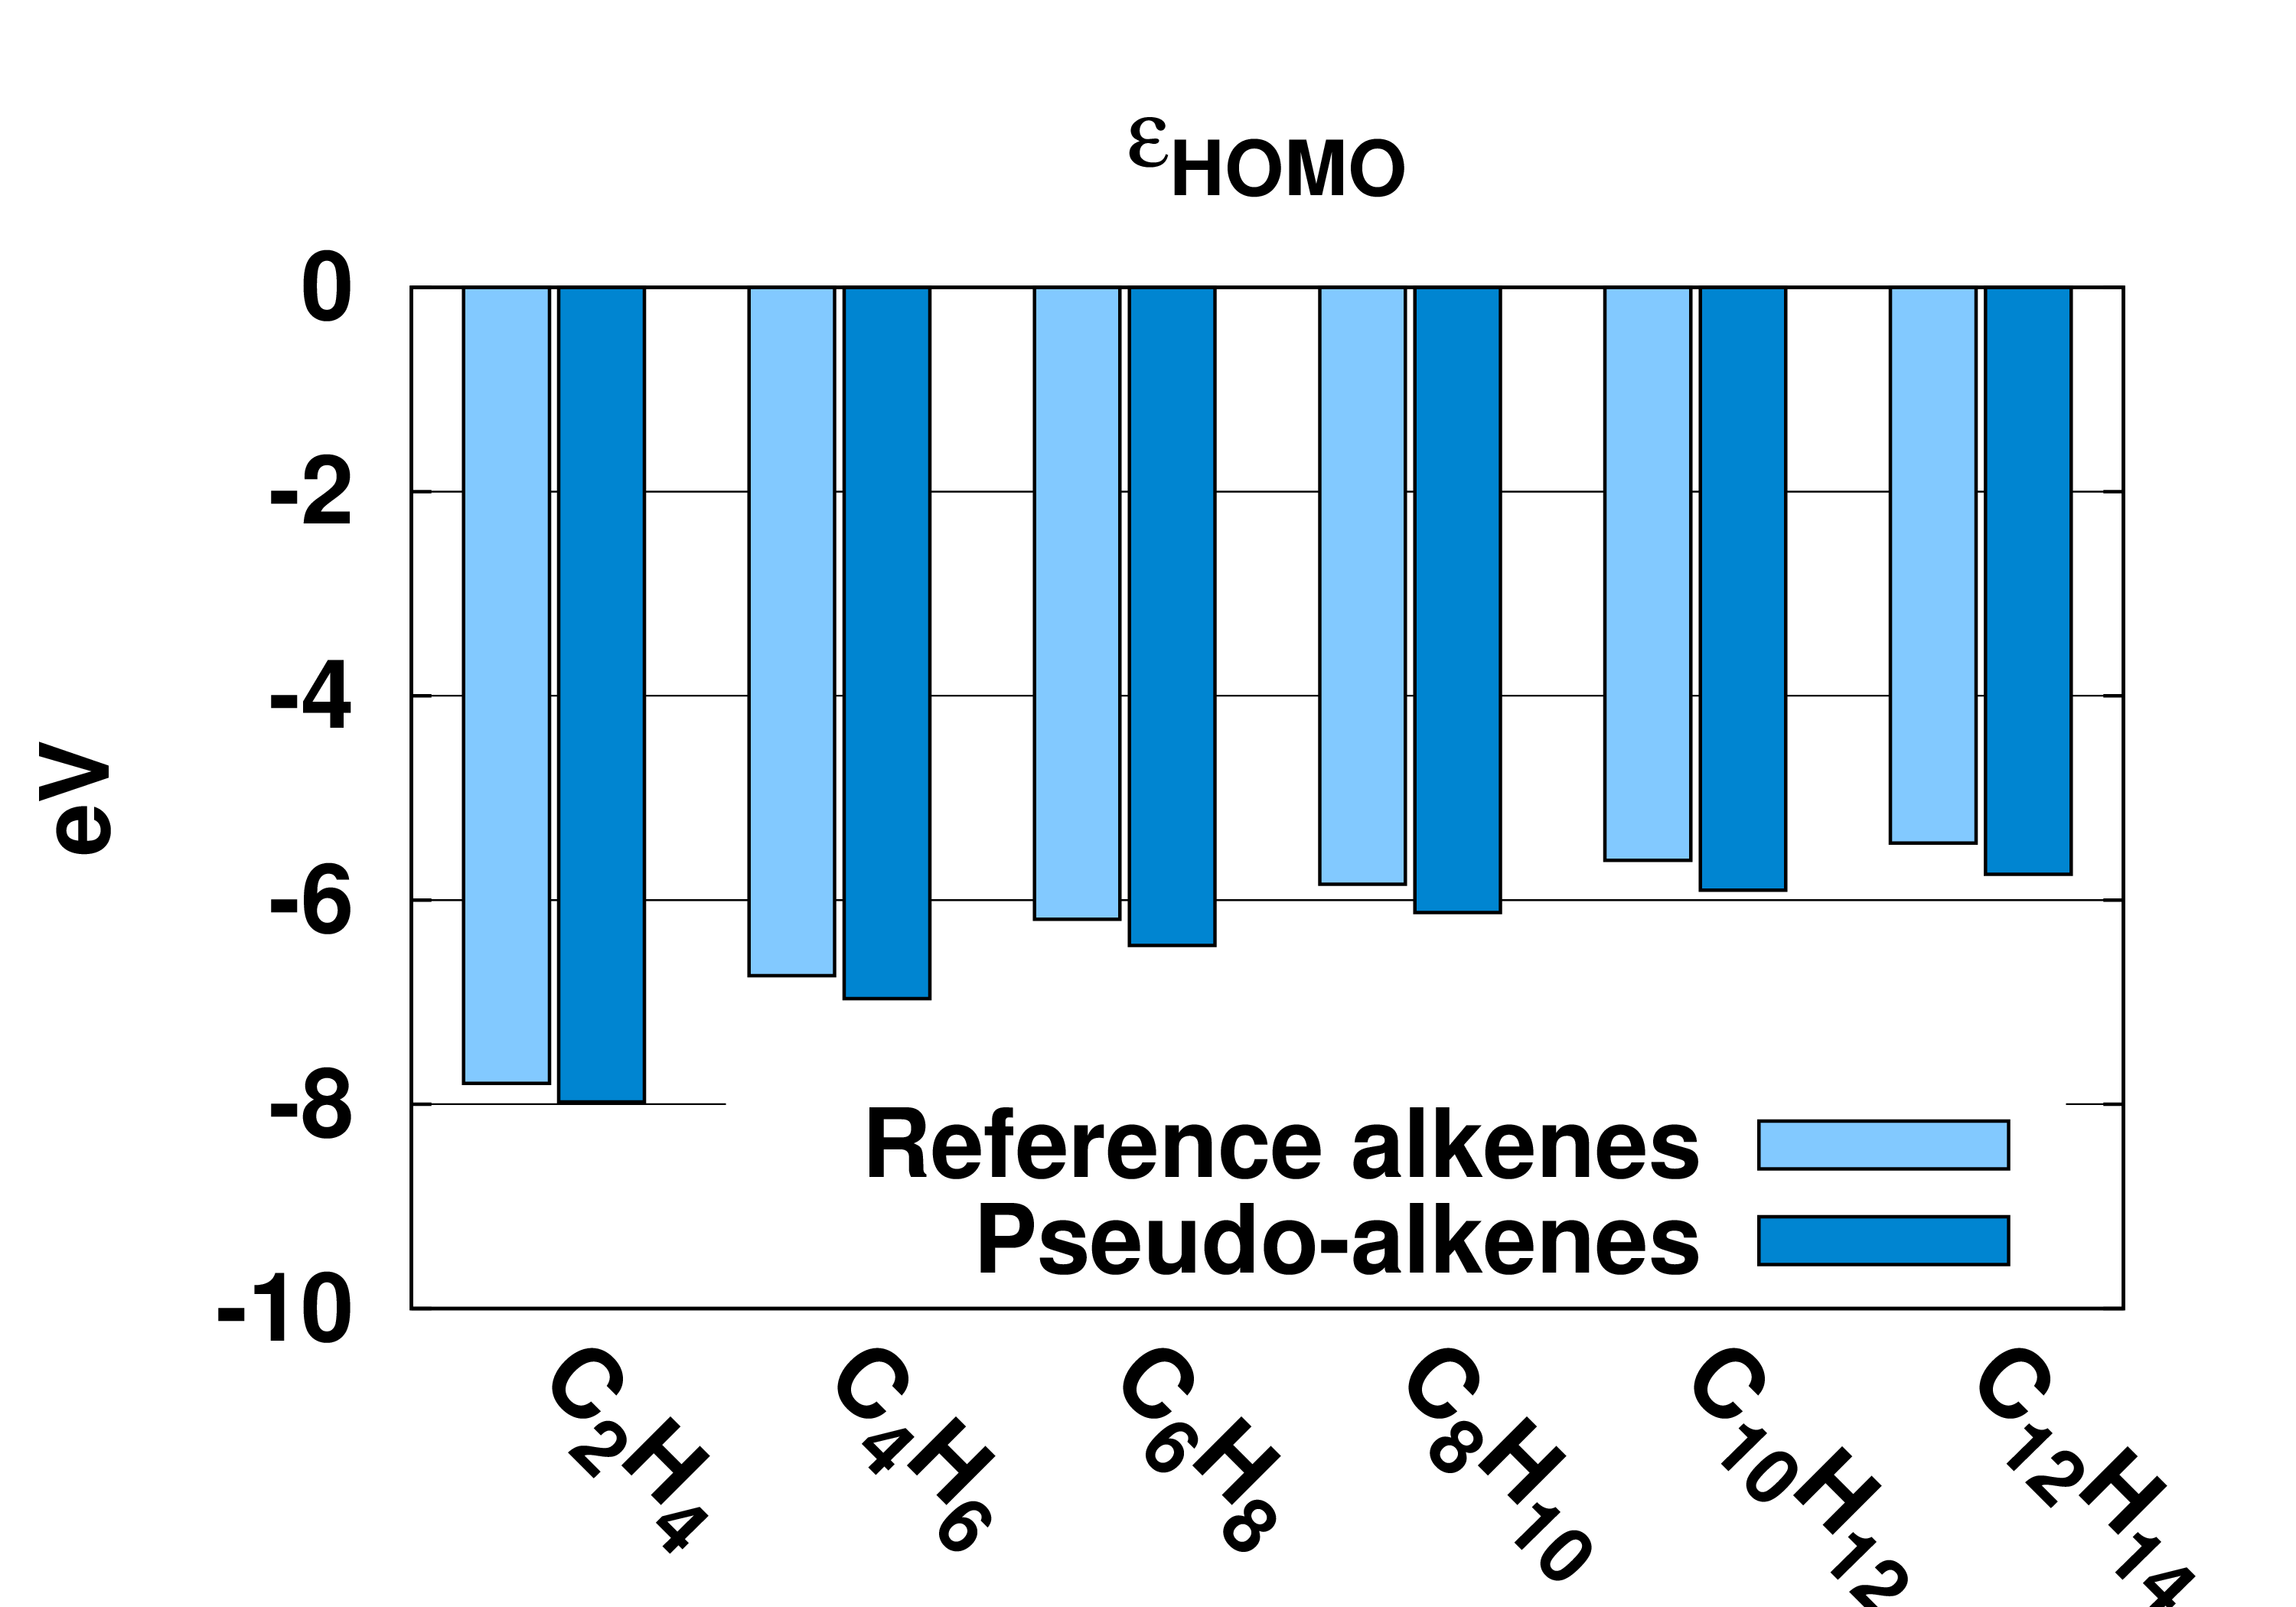
\includegraphics[width=8cm]{short_pbe0_homo}
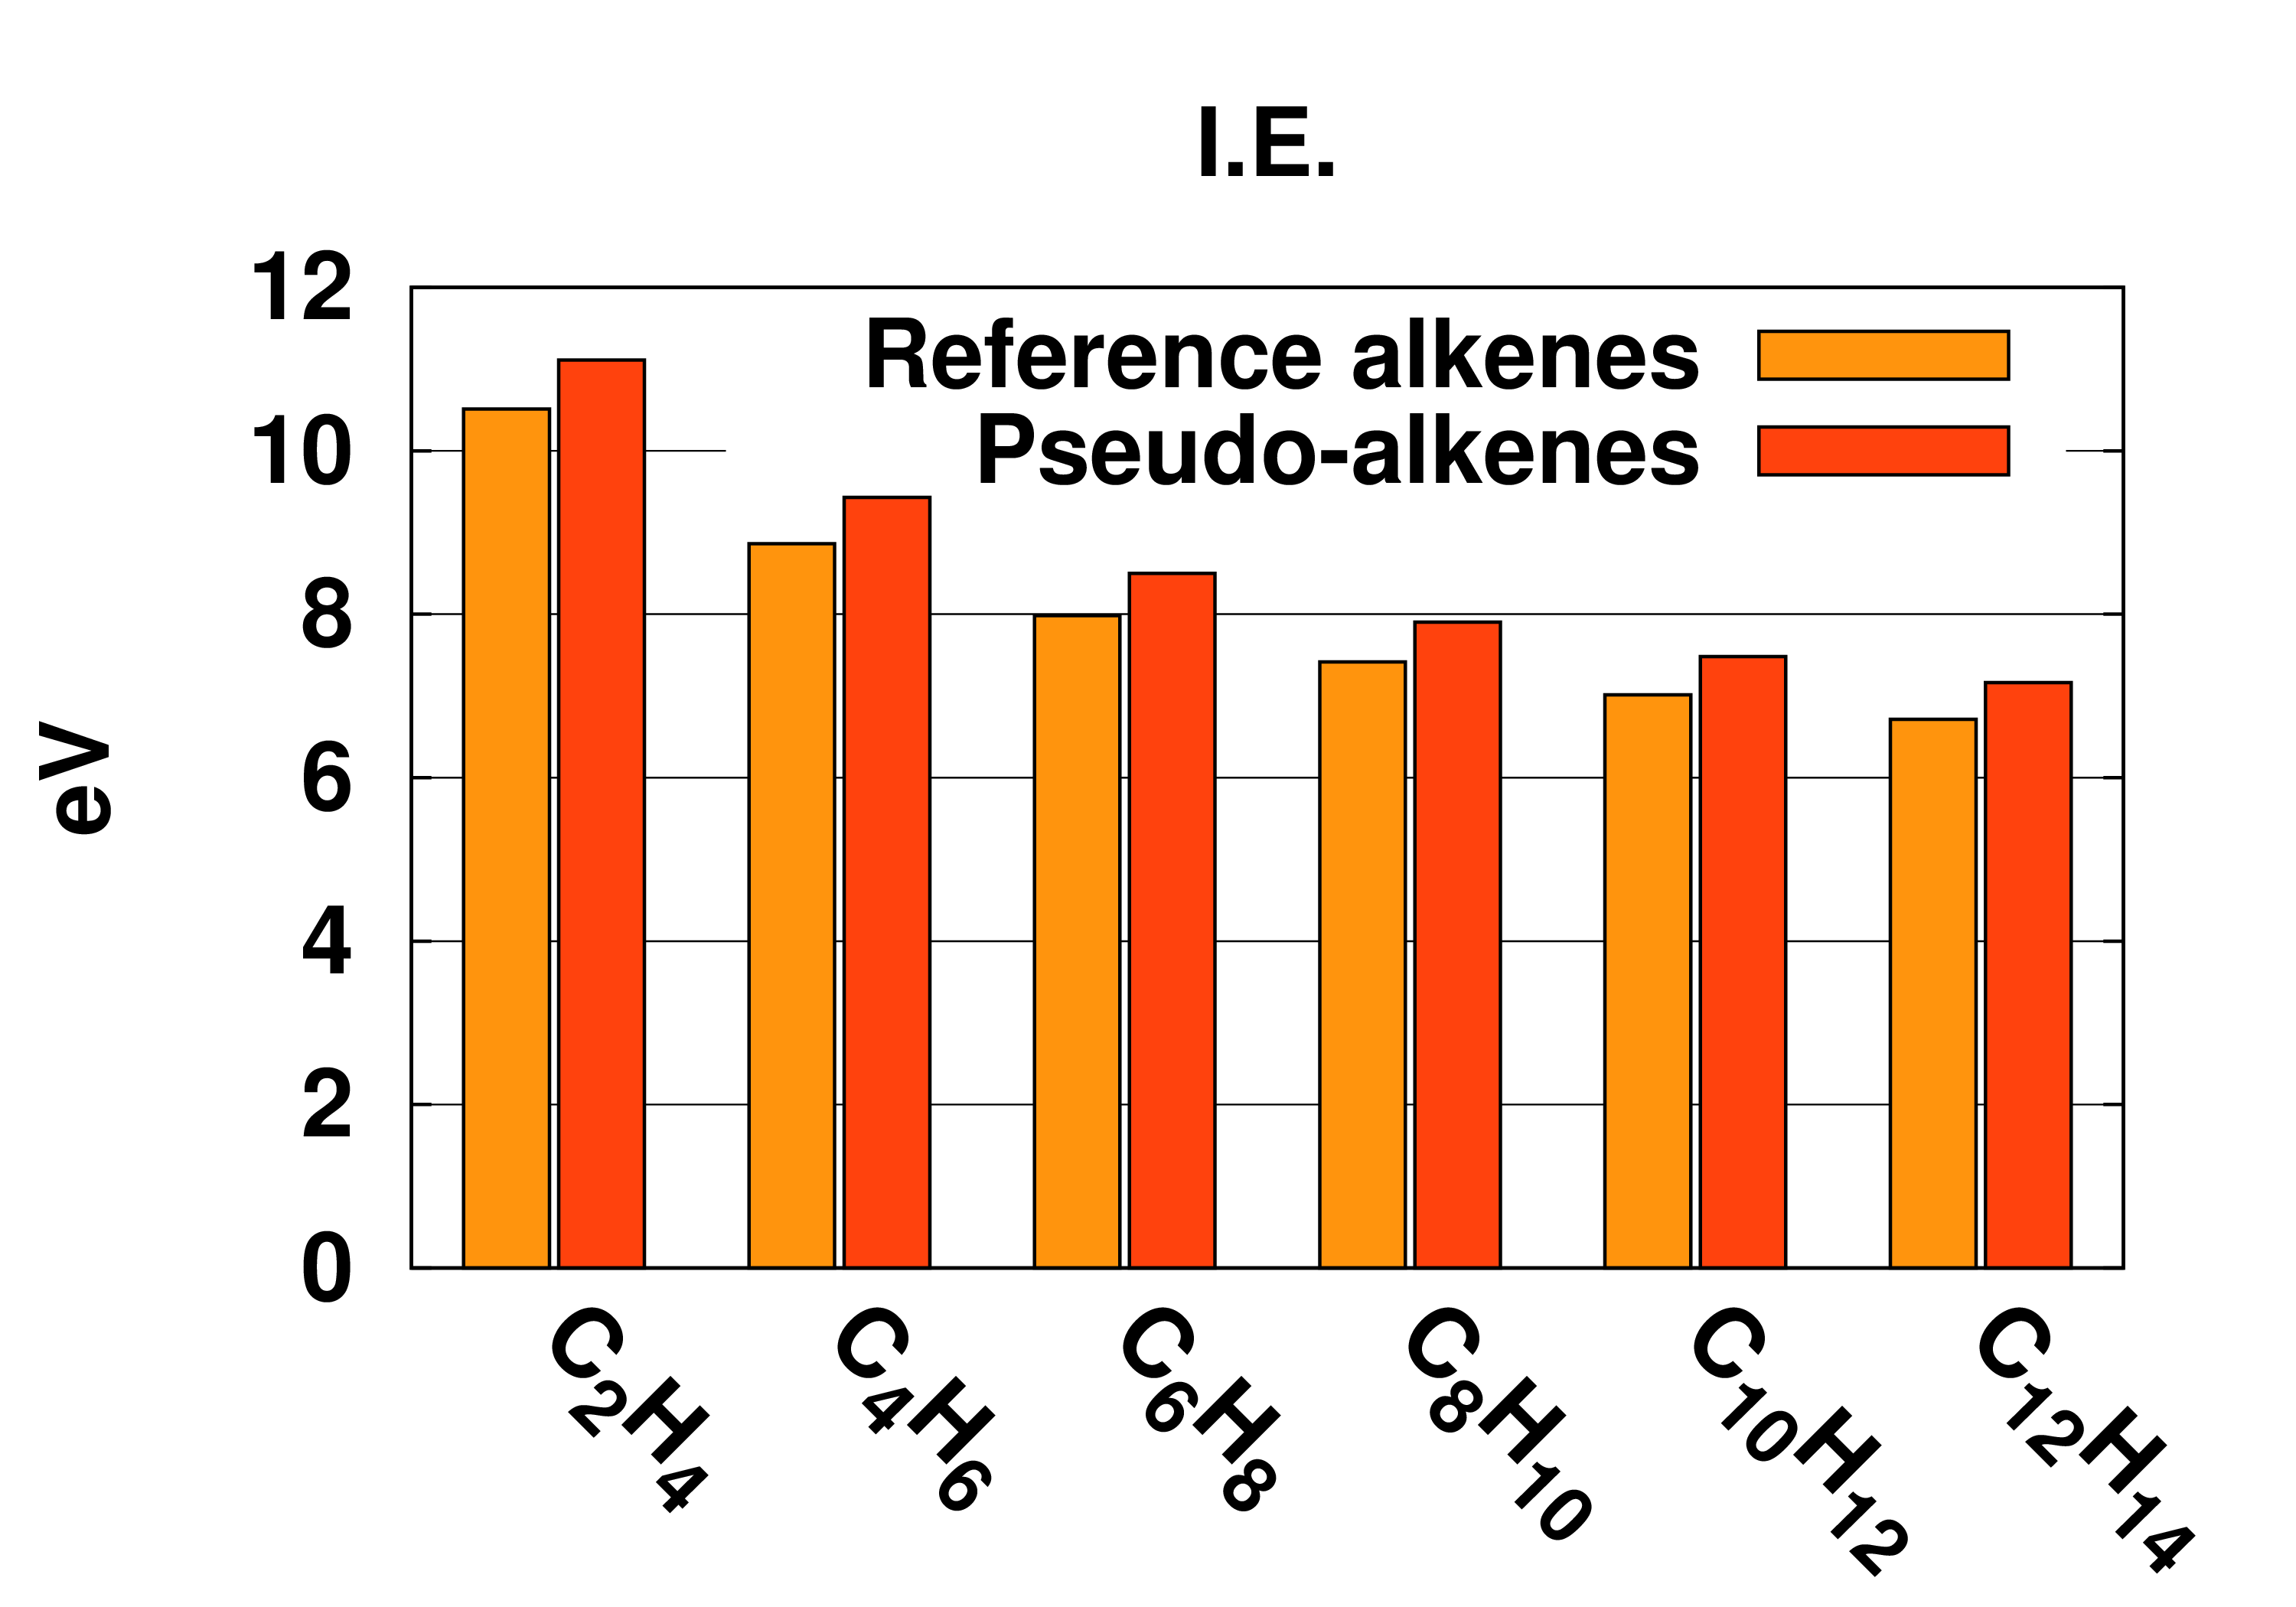
\includegraphics[width=8cm]{short_pbe0_ie}
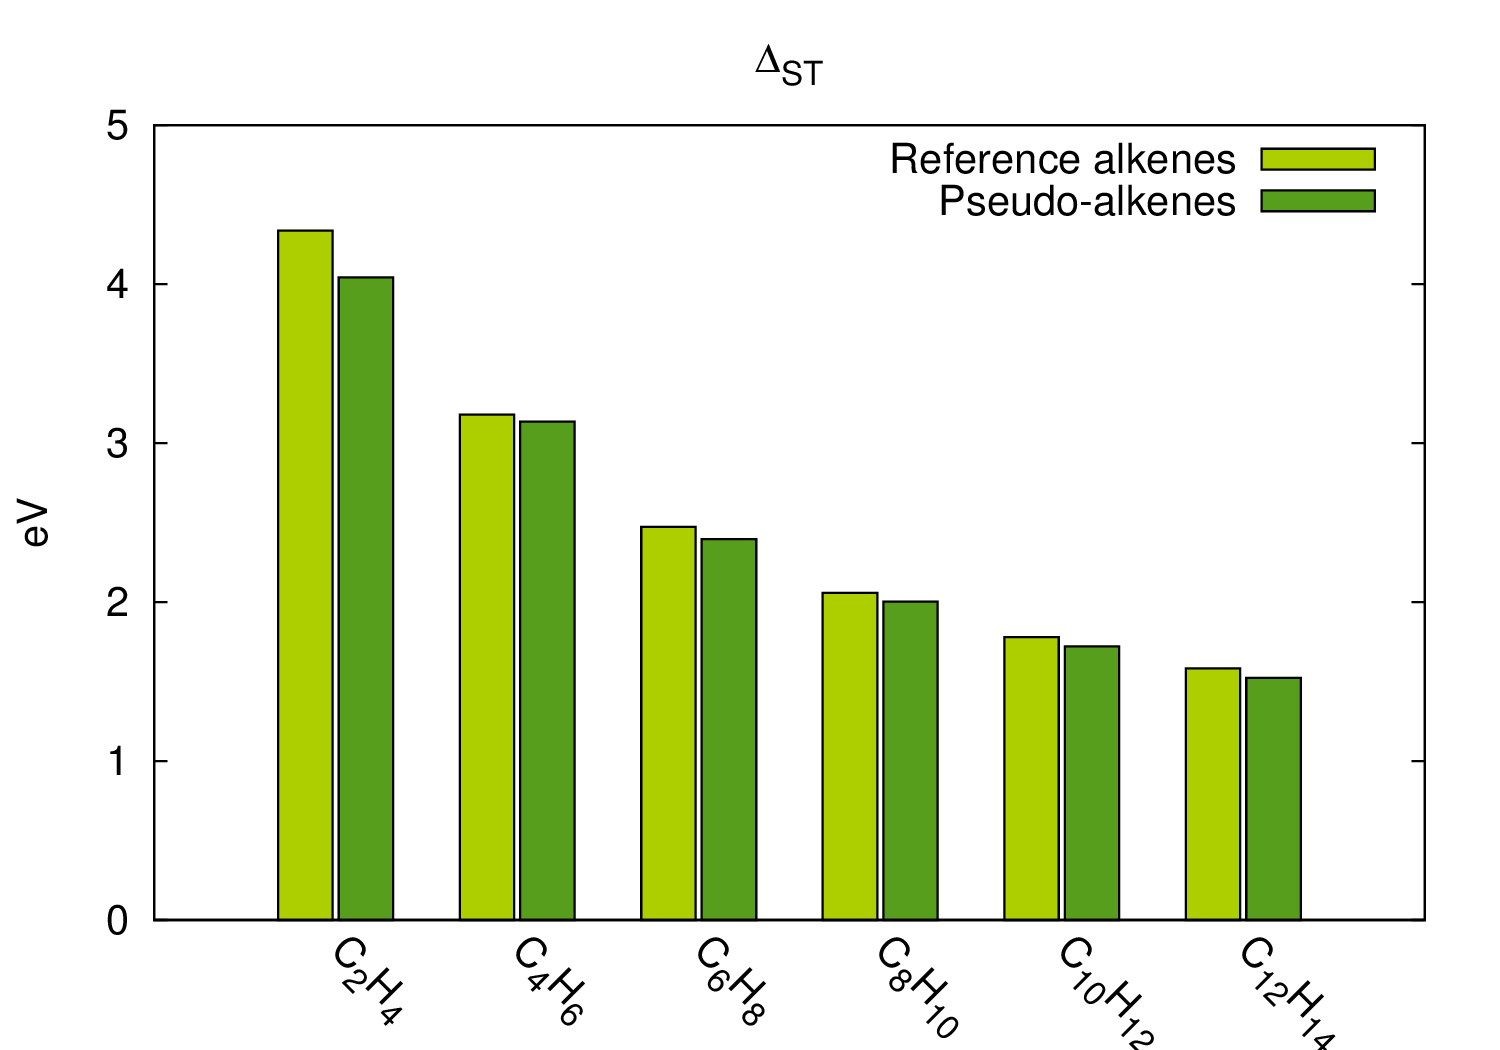
\includegraphics[width=8cm]{short_pbe0_st}
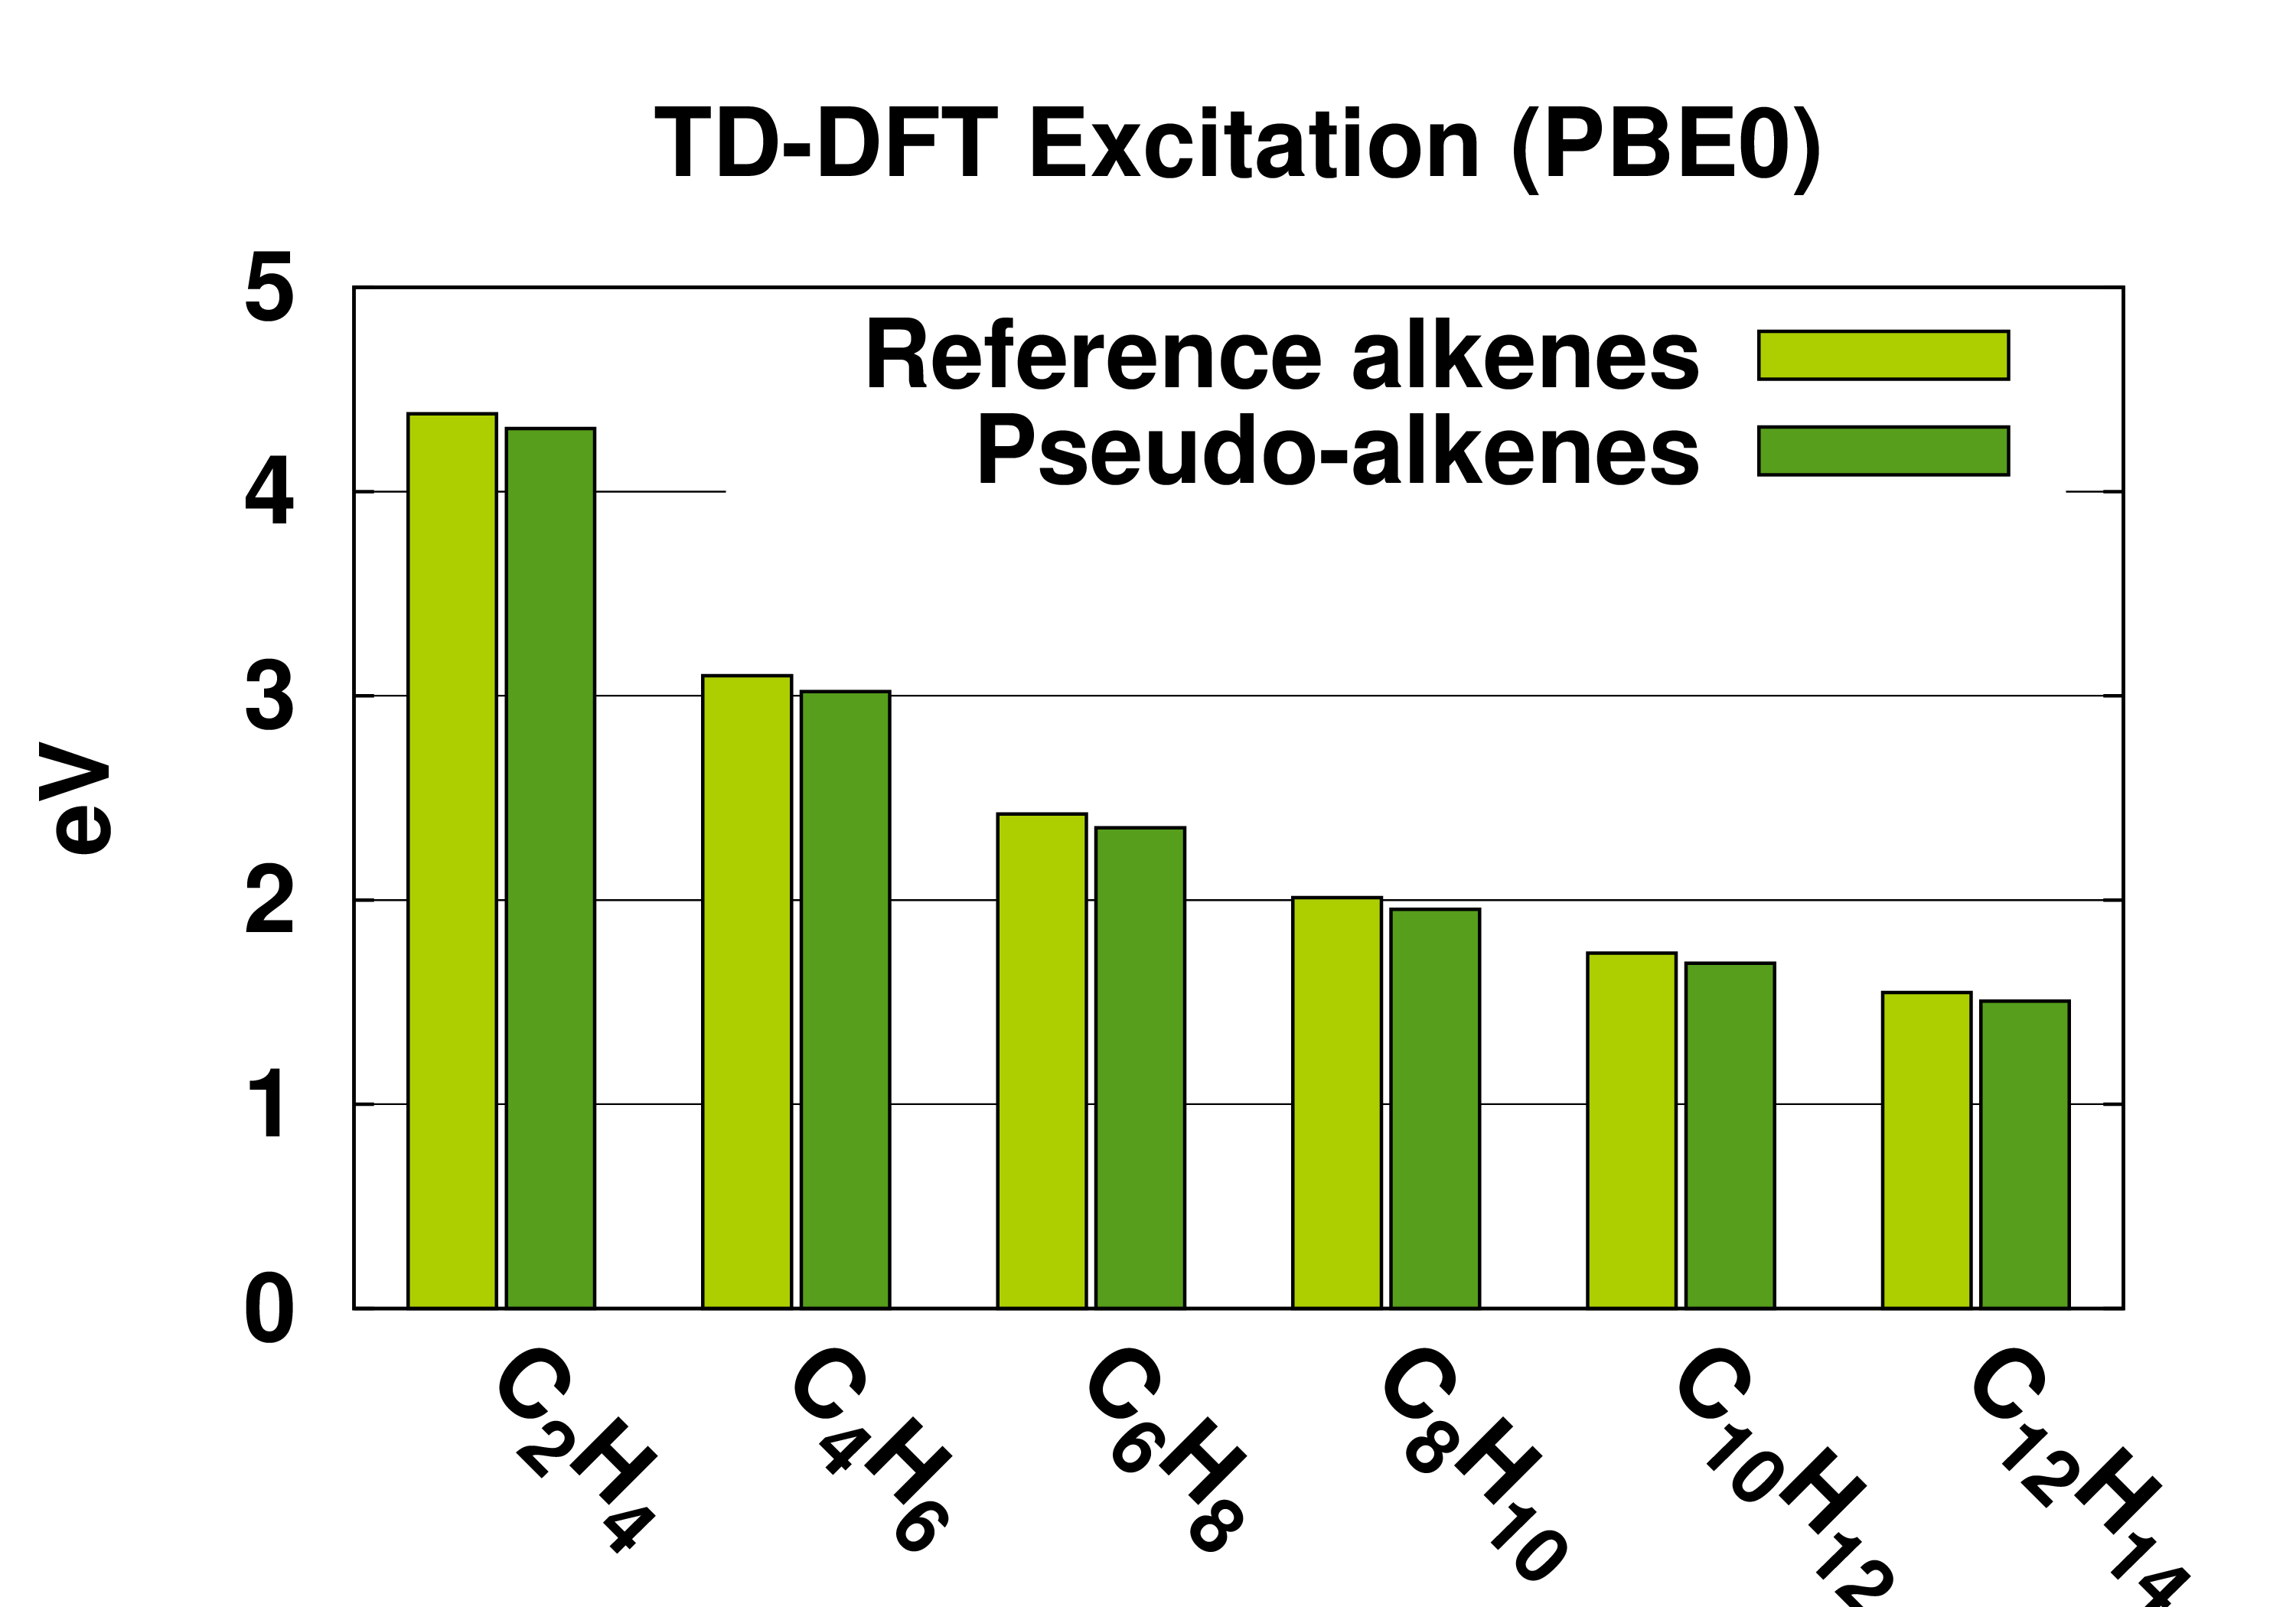
\includegraphics[width=8cm]{short_pbe0_tddft}
\end{center}
\caption{Comparison of the HOMO energy ($\varepsilon_{HOMO}$),
the ionisation energy (I.E.),
the first singlet-triplet excitation energy ($\Delta_{ST}$) and
the TD-DFT first excitation energy
between the
all electron reference system and the optimal pseudo-potential across a range of chain alkenes.
The $\Delta_{ST}$ values were obtained as the difference
between the lowest triplet (in an unrestricted formalism) and the lowest singlet state
(in a restricted formalism).
Calculations were done at the PBE0/def-SV(P) level.}
\label{fig:alkenes_hf_dft}
\end{figure}

\begin{table}[ht]
\begin{tabular}{l r r r r r }
\hline \hline
                        & HF & PBE0 & PBE & TPSS & TPSSh \\
\hline
$\varepsilon_{HOMO}$    & 1.3 & 4.0 & 8.5 & 12.0 &  9.7 \\
I.E.                    & 5.3 & 6.0 & 8.1 & 10.1 &  9.0 \\
$\Delta_{ST}$           & 4.1 & 3.6 & 7.5 & 13.3 & 11.4 \\
TD-DFT First Excitation &   - & 2.6 &   - &    - &    - \\ 
\hline\hline
\end{tabular}
\caption{Mean relative errors (in percent) across methods (HF or different functionals)
for short chain alkenes  (C\(_{2}\)-C\(_{12}\)).}
\label{table:alkene_errors}
\end{table}

Also compared are TD-DFT results for this system and results of a previous work of some of the authors, which match to within 3\%.\cite{drujon_pseudopotentials_2013}
Let us recall here that in our previous work potentials were placed at the center of bonds.

\subsection{Larger chains and fused rings}

\begin{figure}
\begin{center}
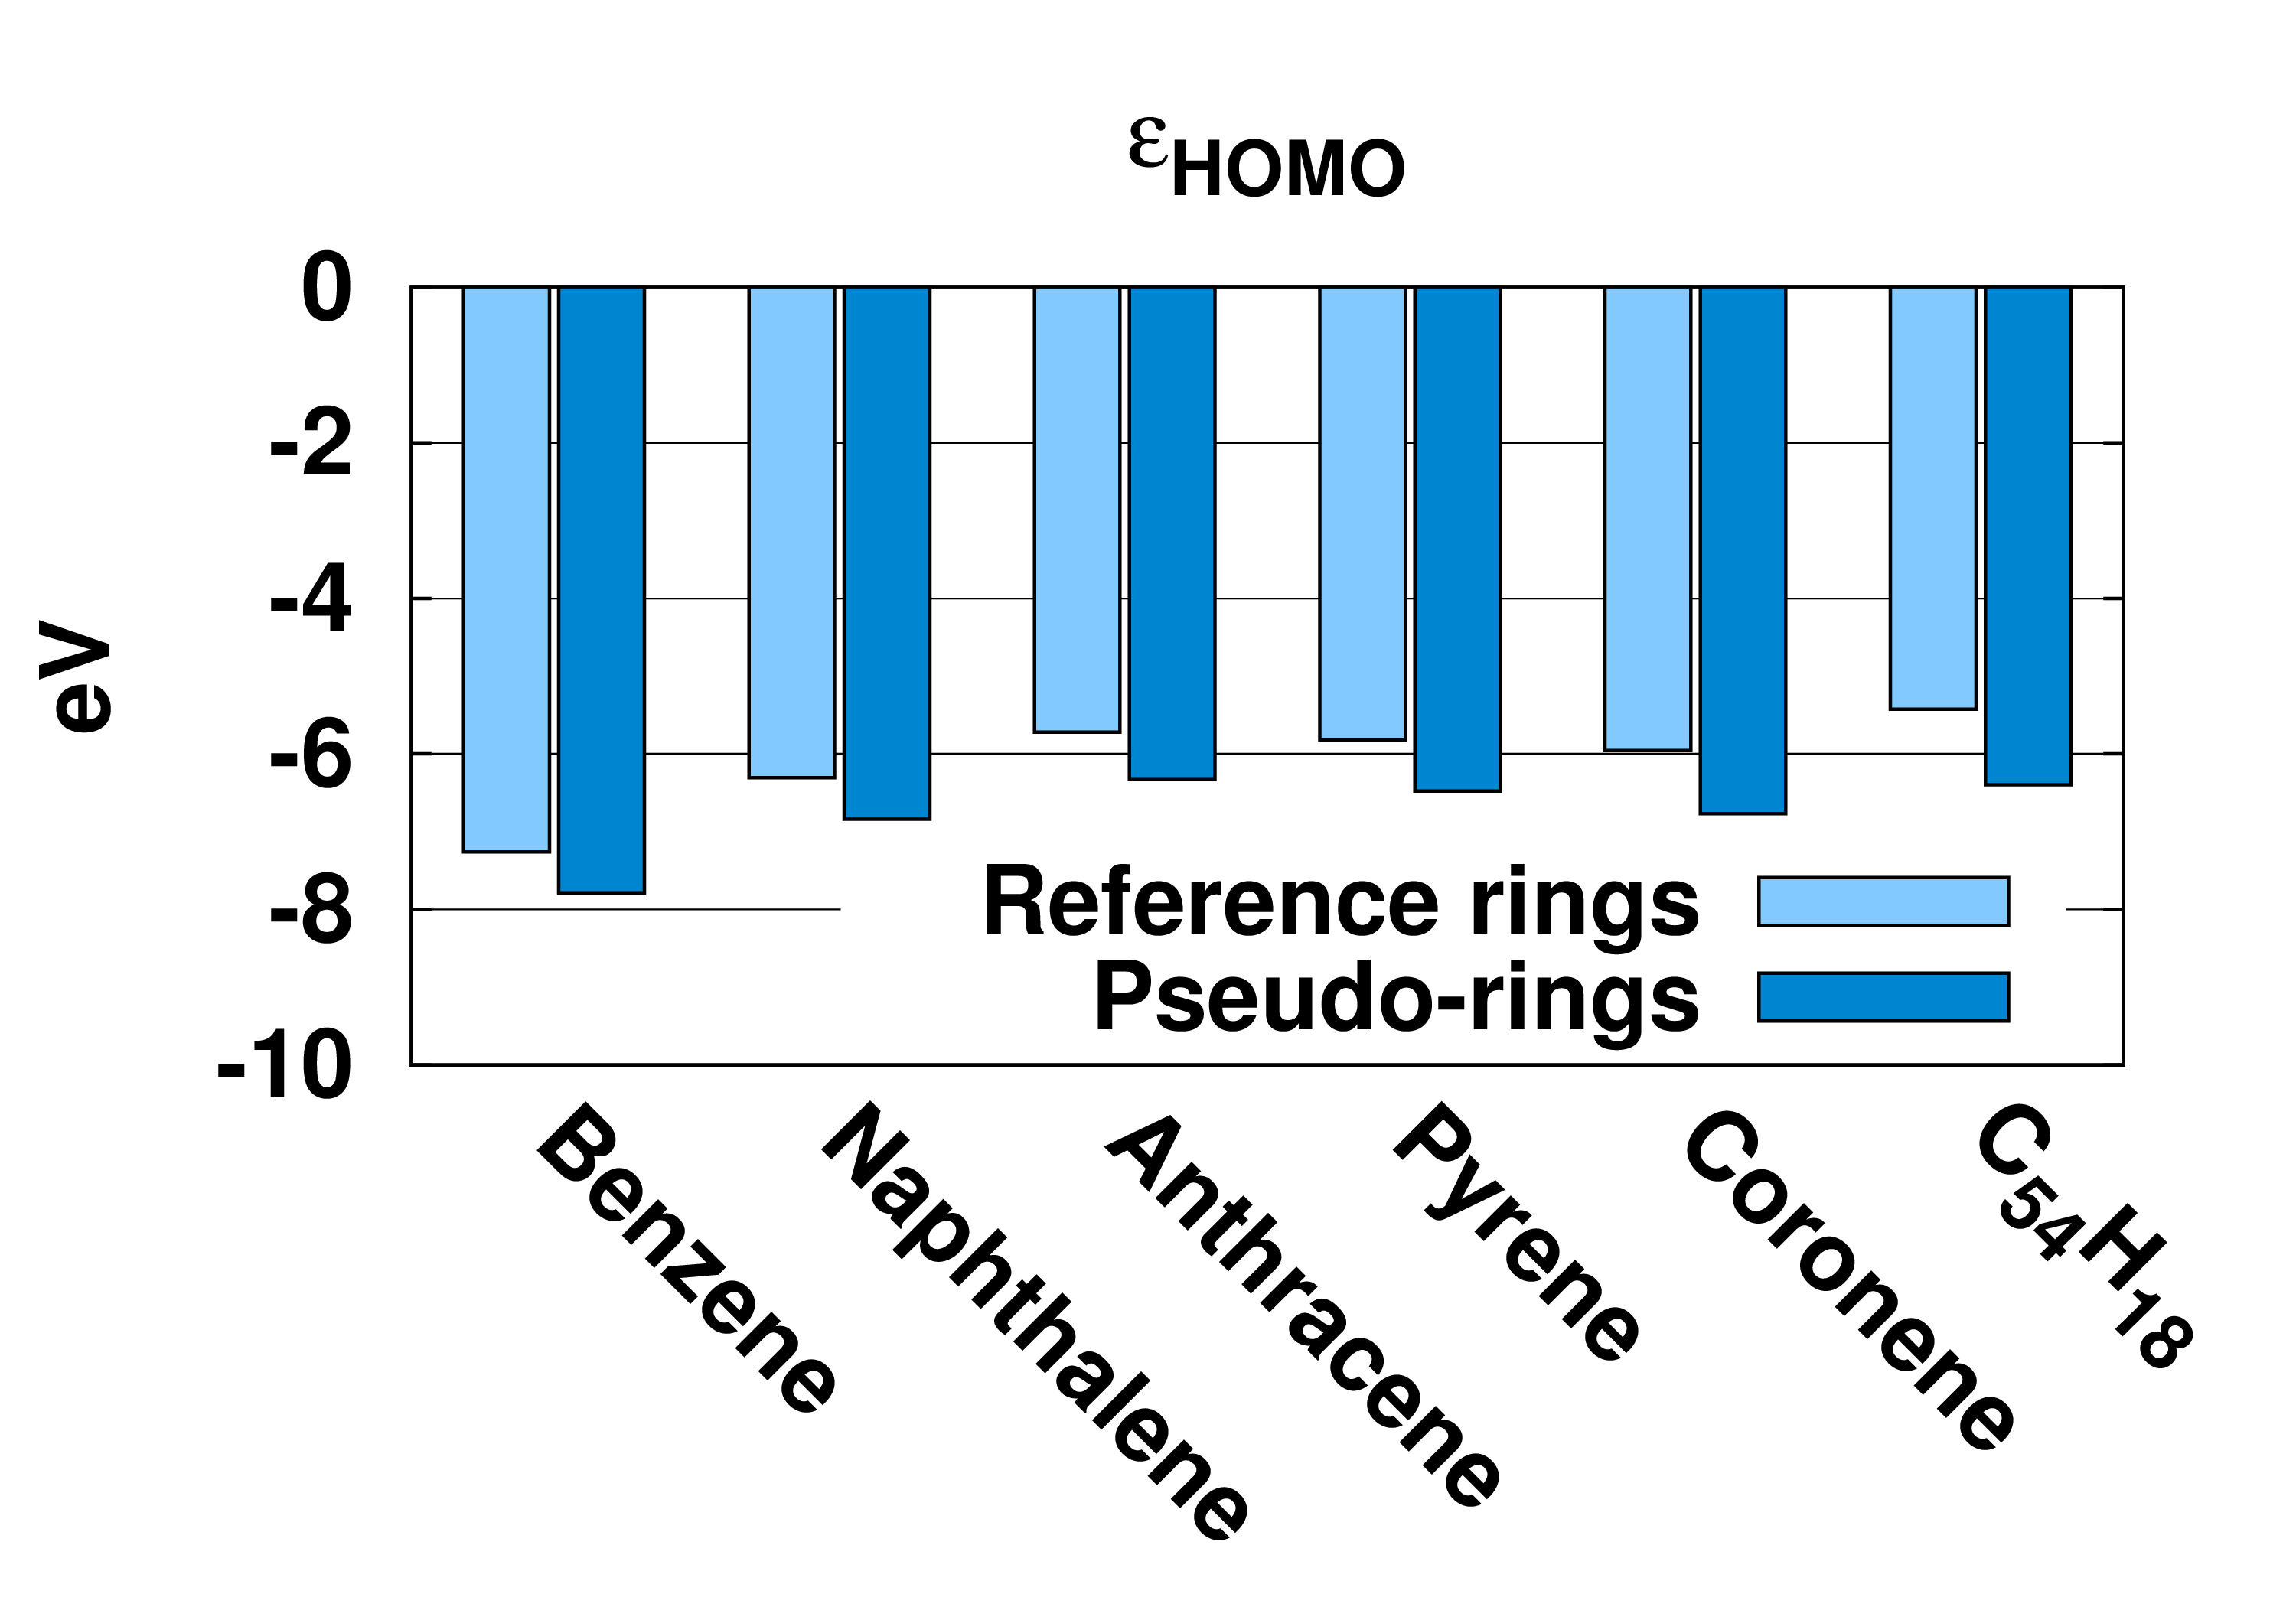
\includegraphics[width=8cm]{ring_pbe0_homo}
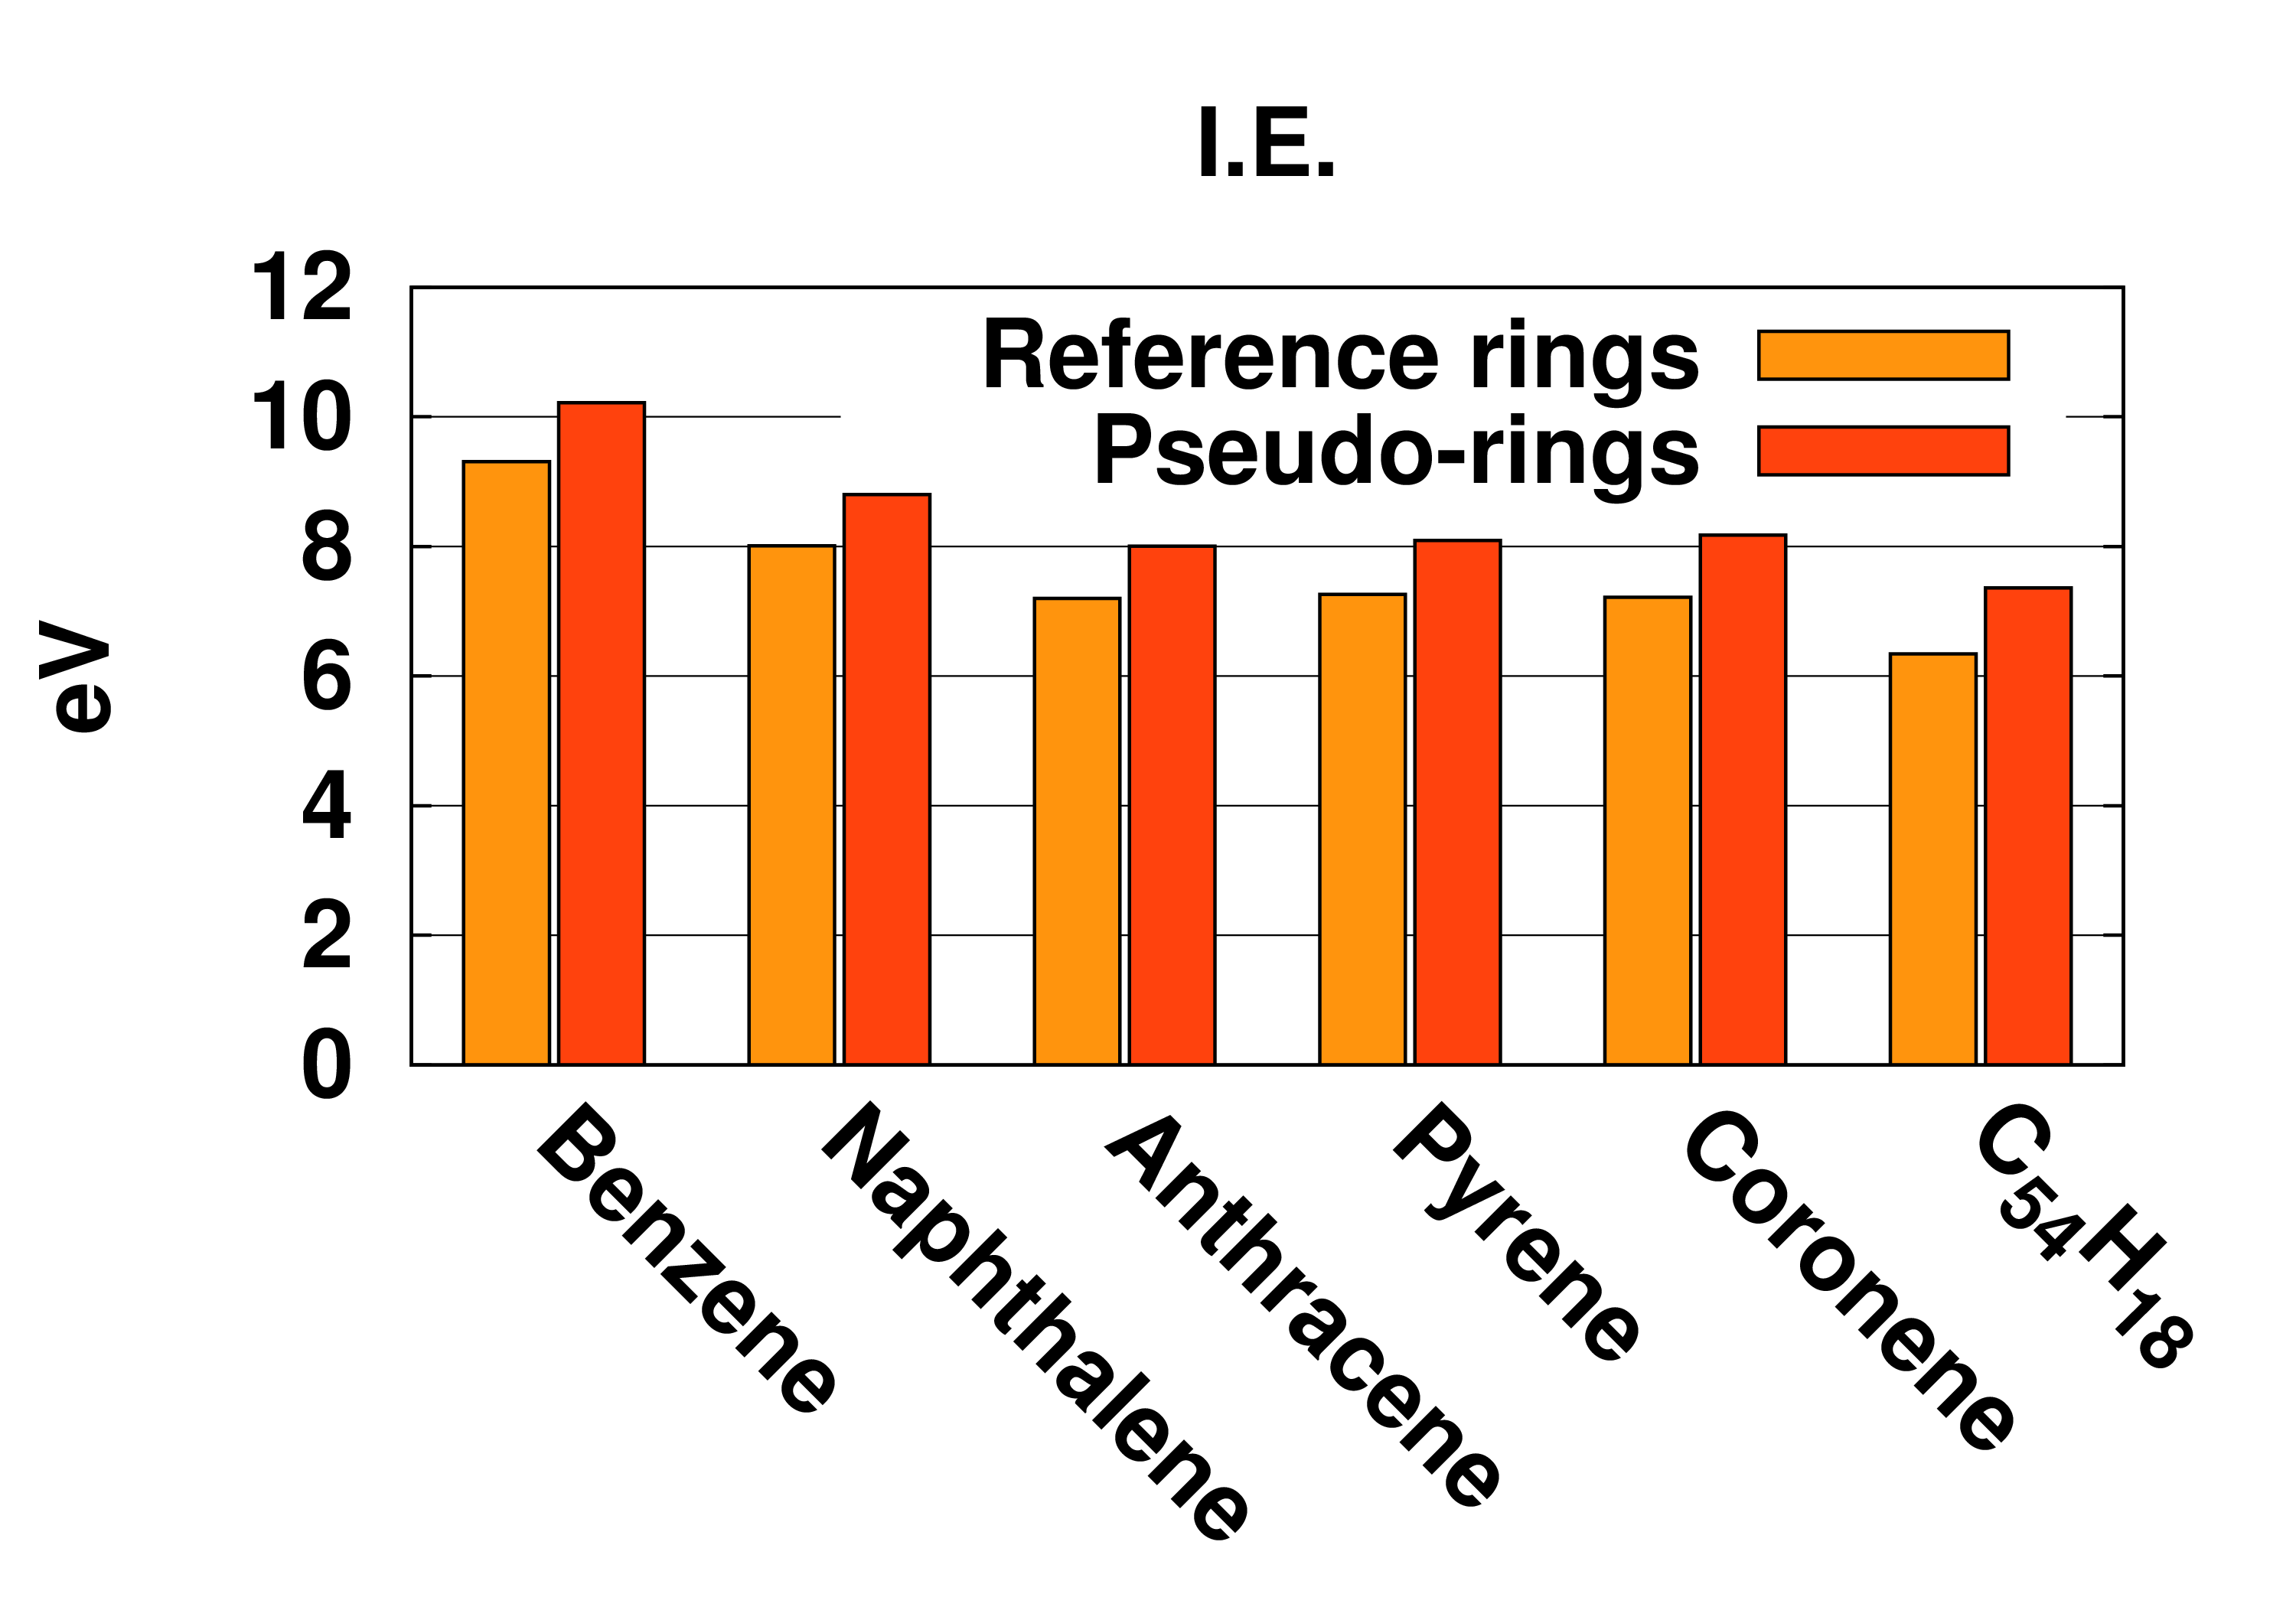
\includegraphics[width=8cm]{ring_pbe0_ie}
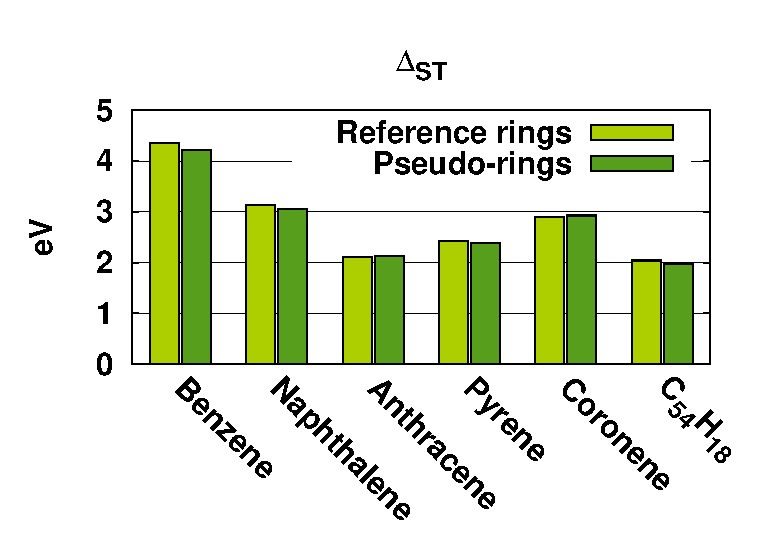
\includegraphics[width=8cm]{ring_pbe0_st}
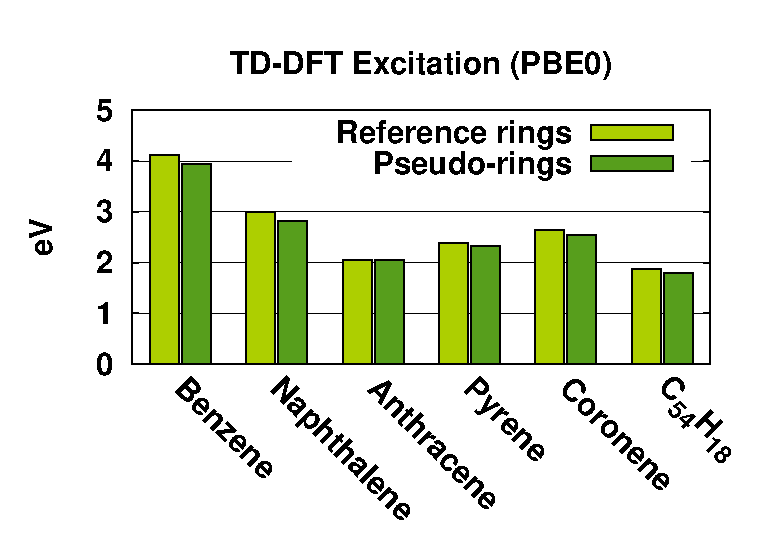
\includegraphics[width=8cm]{ring_pbe0_tddft}
\end{center}

\caption{Comparison of the HOMO energy ($\varepsilon_{HOMO}$),
the ionisation energy (I.E.),
the first singlet-triplet excitation energy ($\Delta_{ST}$) and
the TD-DFT first excitation energy
between the
all electron reference system and the optimal pseudo-potential across a range of ring molecules.
The $\Delta_{ST}$ values were obtained as the difference
between the lowest triplet (in an unrestricted formalism) and the lowest singlet state
(in a restricted formalism).
Calculations were done at the PBE0/def-SV(P) level.
The C\(_{54}\)H\(_{18}\) molecule is represented in figure \ref{fig:c54h18}}
\label{fig:rings_graphs}
\end{figure}

\begin{figure}
\begin{center}
\fbox{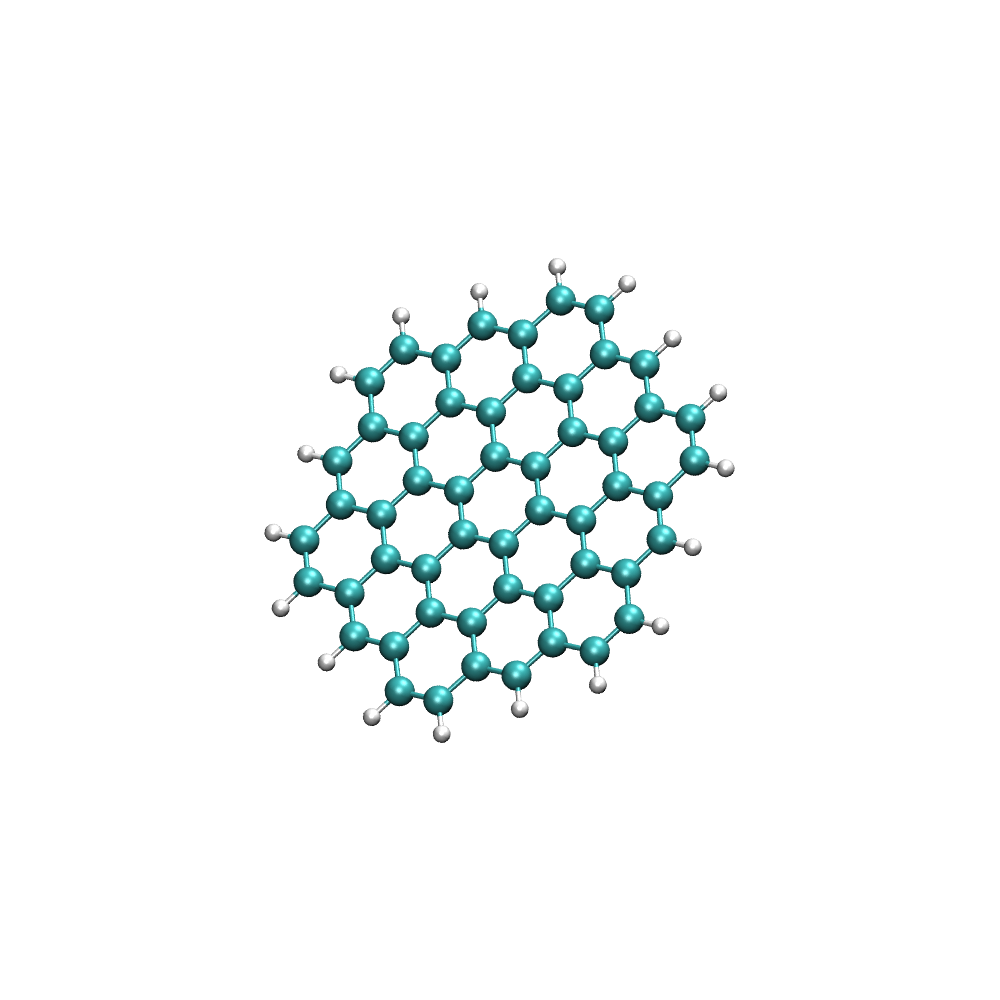
\includegraphics[width=5cm]{c54h18}}
\end{center}
\caption{\label{fig:c54h18}The C\(_{54}\)H\(_{18}\) molecule.}
\end{figure}

The potentials derived above are also tested on larger systems.
Figure \ref{fig:rings_graphs} shows the $\Delta_{ST}$, the IE and
HOMO energy values for several ring systems.
As with the short chain alkenes, the general trend of the results is well-replicated
by the pseudo-systems, and the percentage errors, displayed in Table
\ref{table:ring_system_errors}, are similar.

\begin{table}[ht]
\begin{tabular}{l r r r r r }
\hline\hline
                        & HF & PBE0 & PBE & TPSS & TPSSH \\
\hline
$\varepsilon_{HOMO}$    & 3.4 &  9.3  & 13.4 & 17.1 & 14.7 \\
I.E.                    & 7.4 & 10.0  & 12.5 & 14.4 & 13.0 \\
$\Delta_{ST}$           & 3.3 &  1.9  &  1.7 &  6.8 &  6.7 \\
TD-DFT First Excitation &   - & 0.099 &    - &    - &    - \\ 
\hline\hline
\end{tabular}
\caption{Mean relative errors (in percent) across methods (HF or different functionals)
for ring-systems.}
\label{table:ring_system_errors}
\end{table}

Figure~\ref{fig:long_chain_graphs} and Table \ref{table:long_alkene_errors} refer to longer 
alkene chains (\(n\) up to 100).

\begin{figure}
\begin{center}
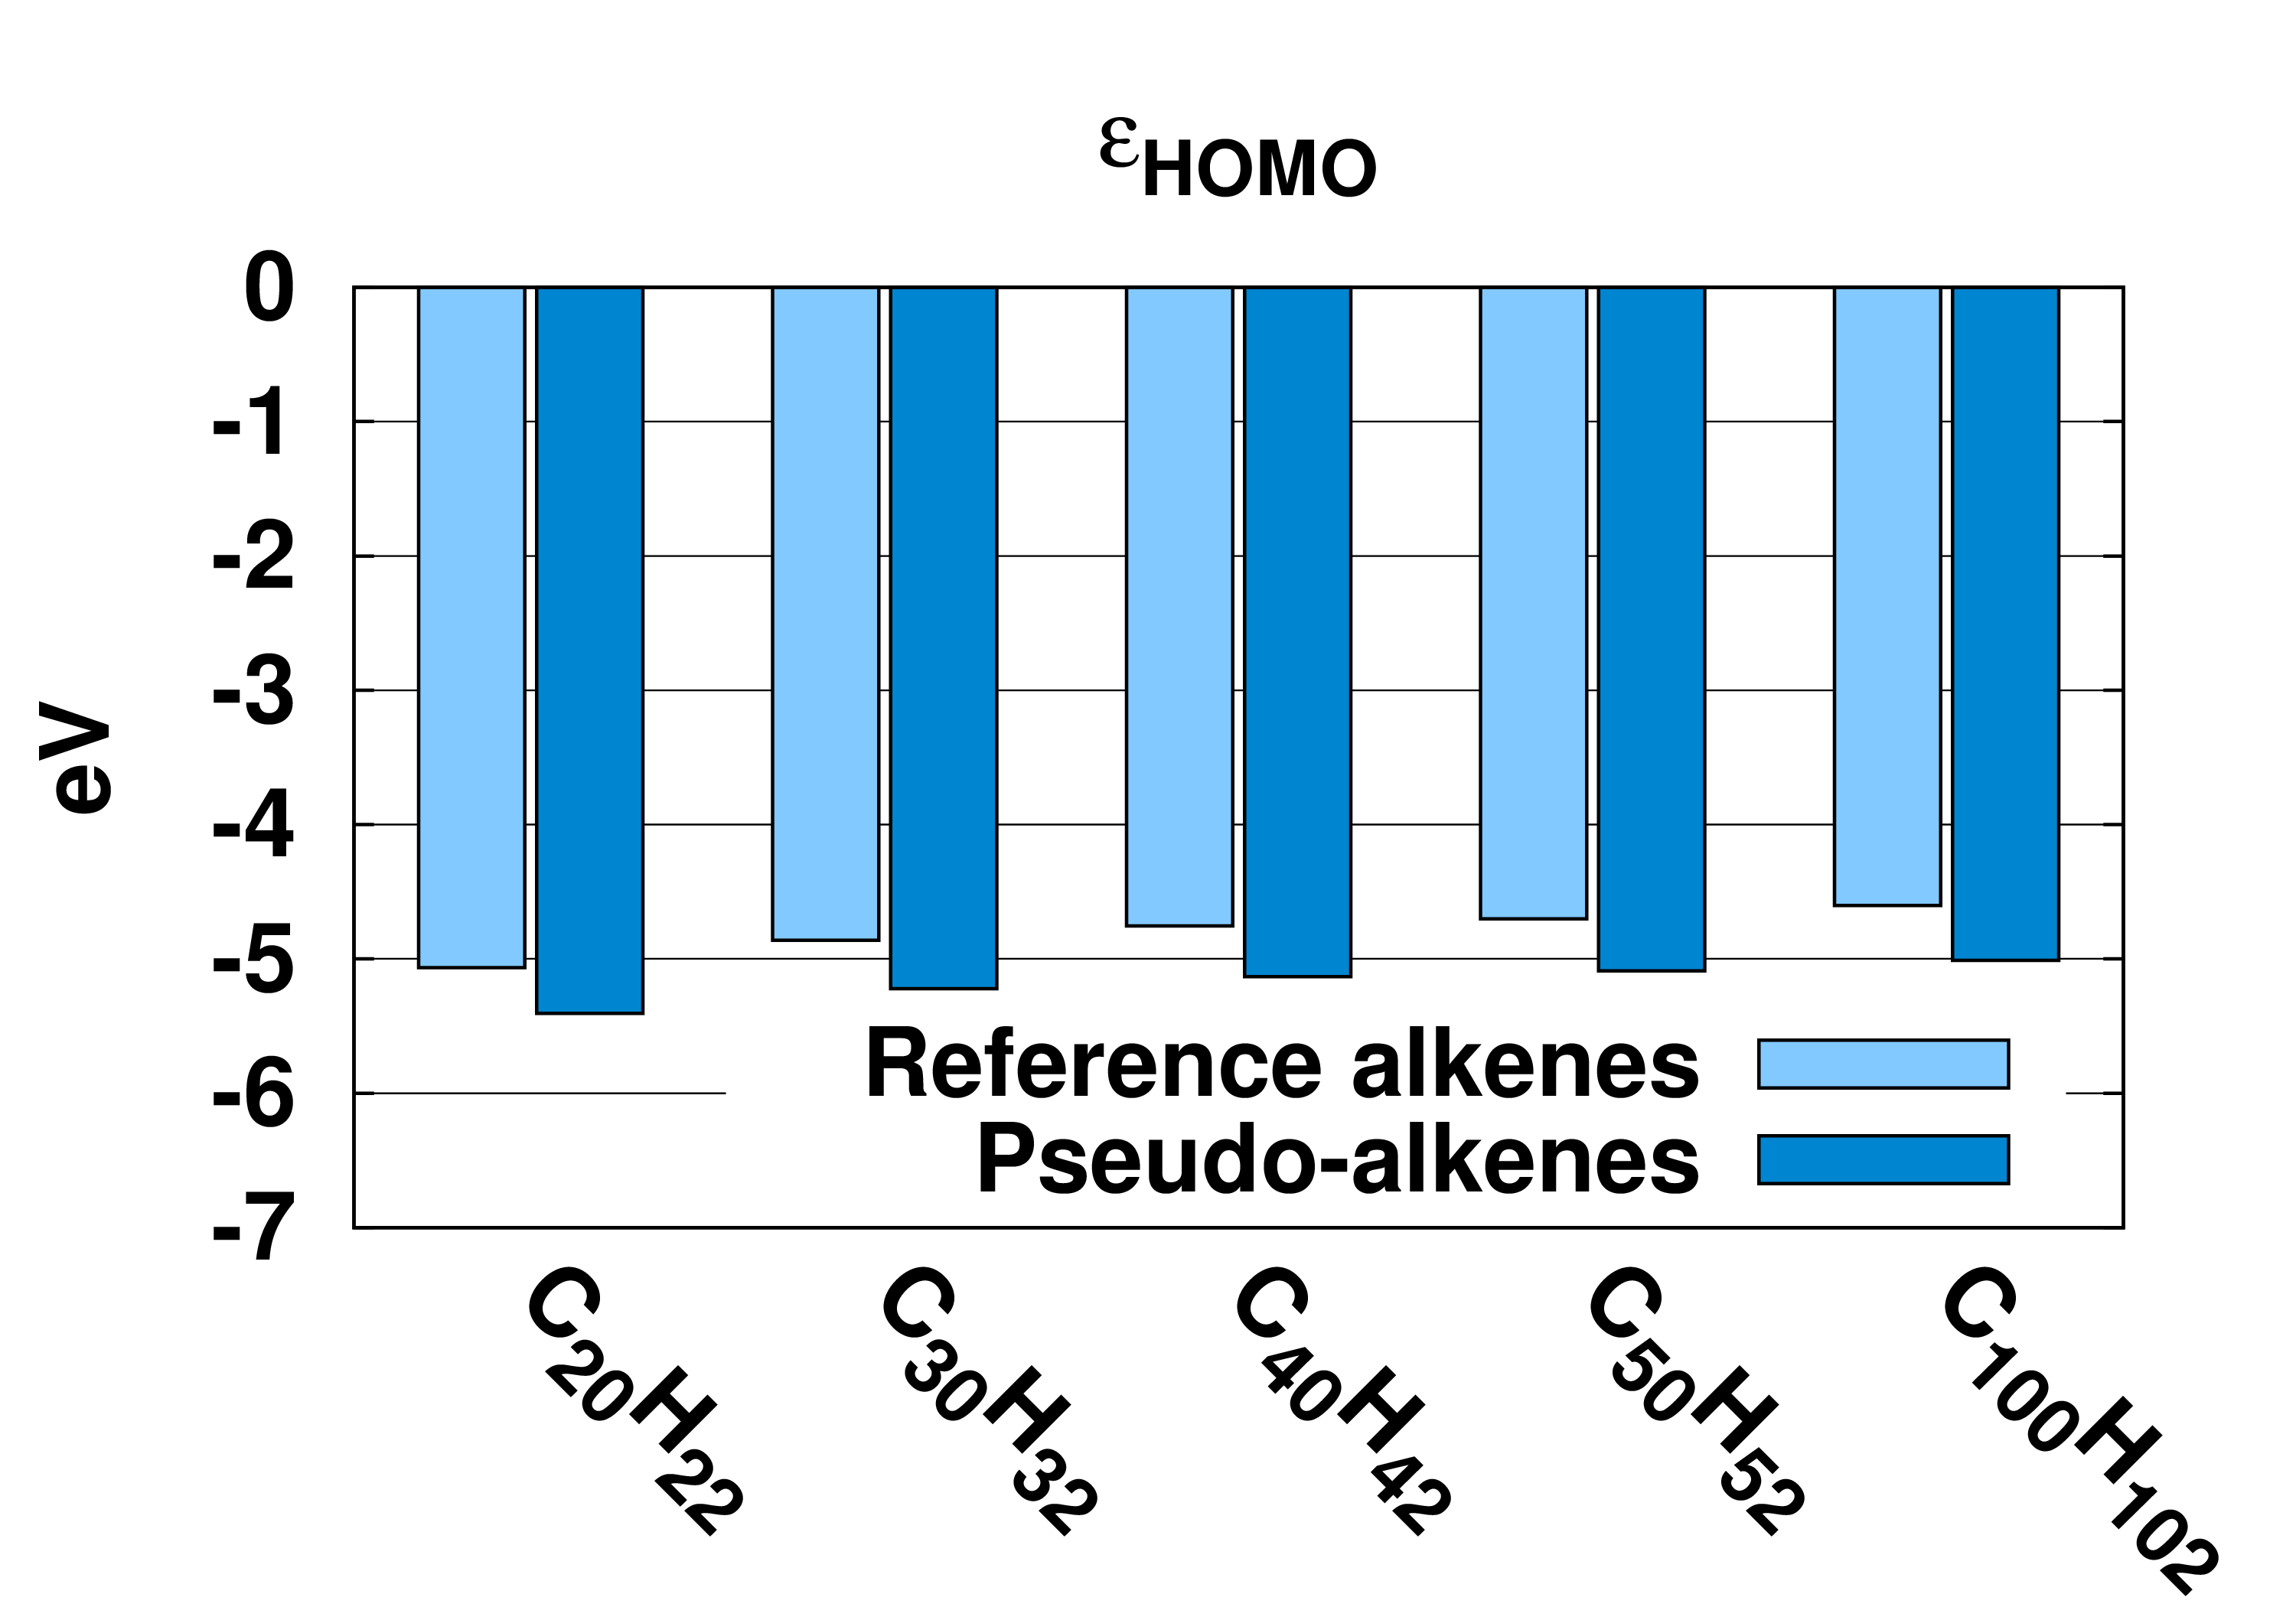
\includegraphics[width=8cm]{long_pbe0_homo}
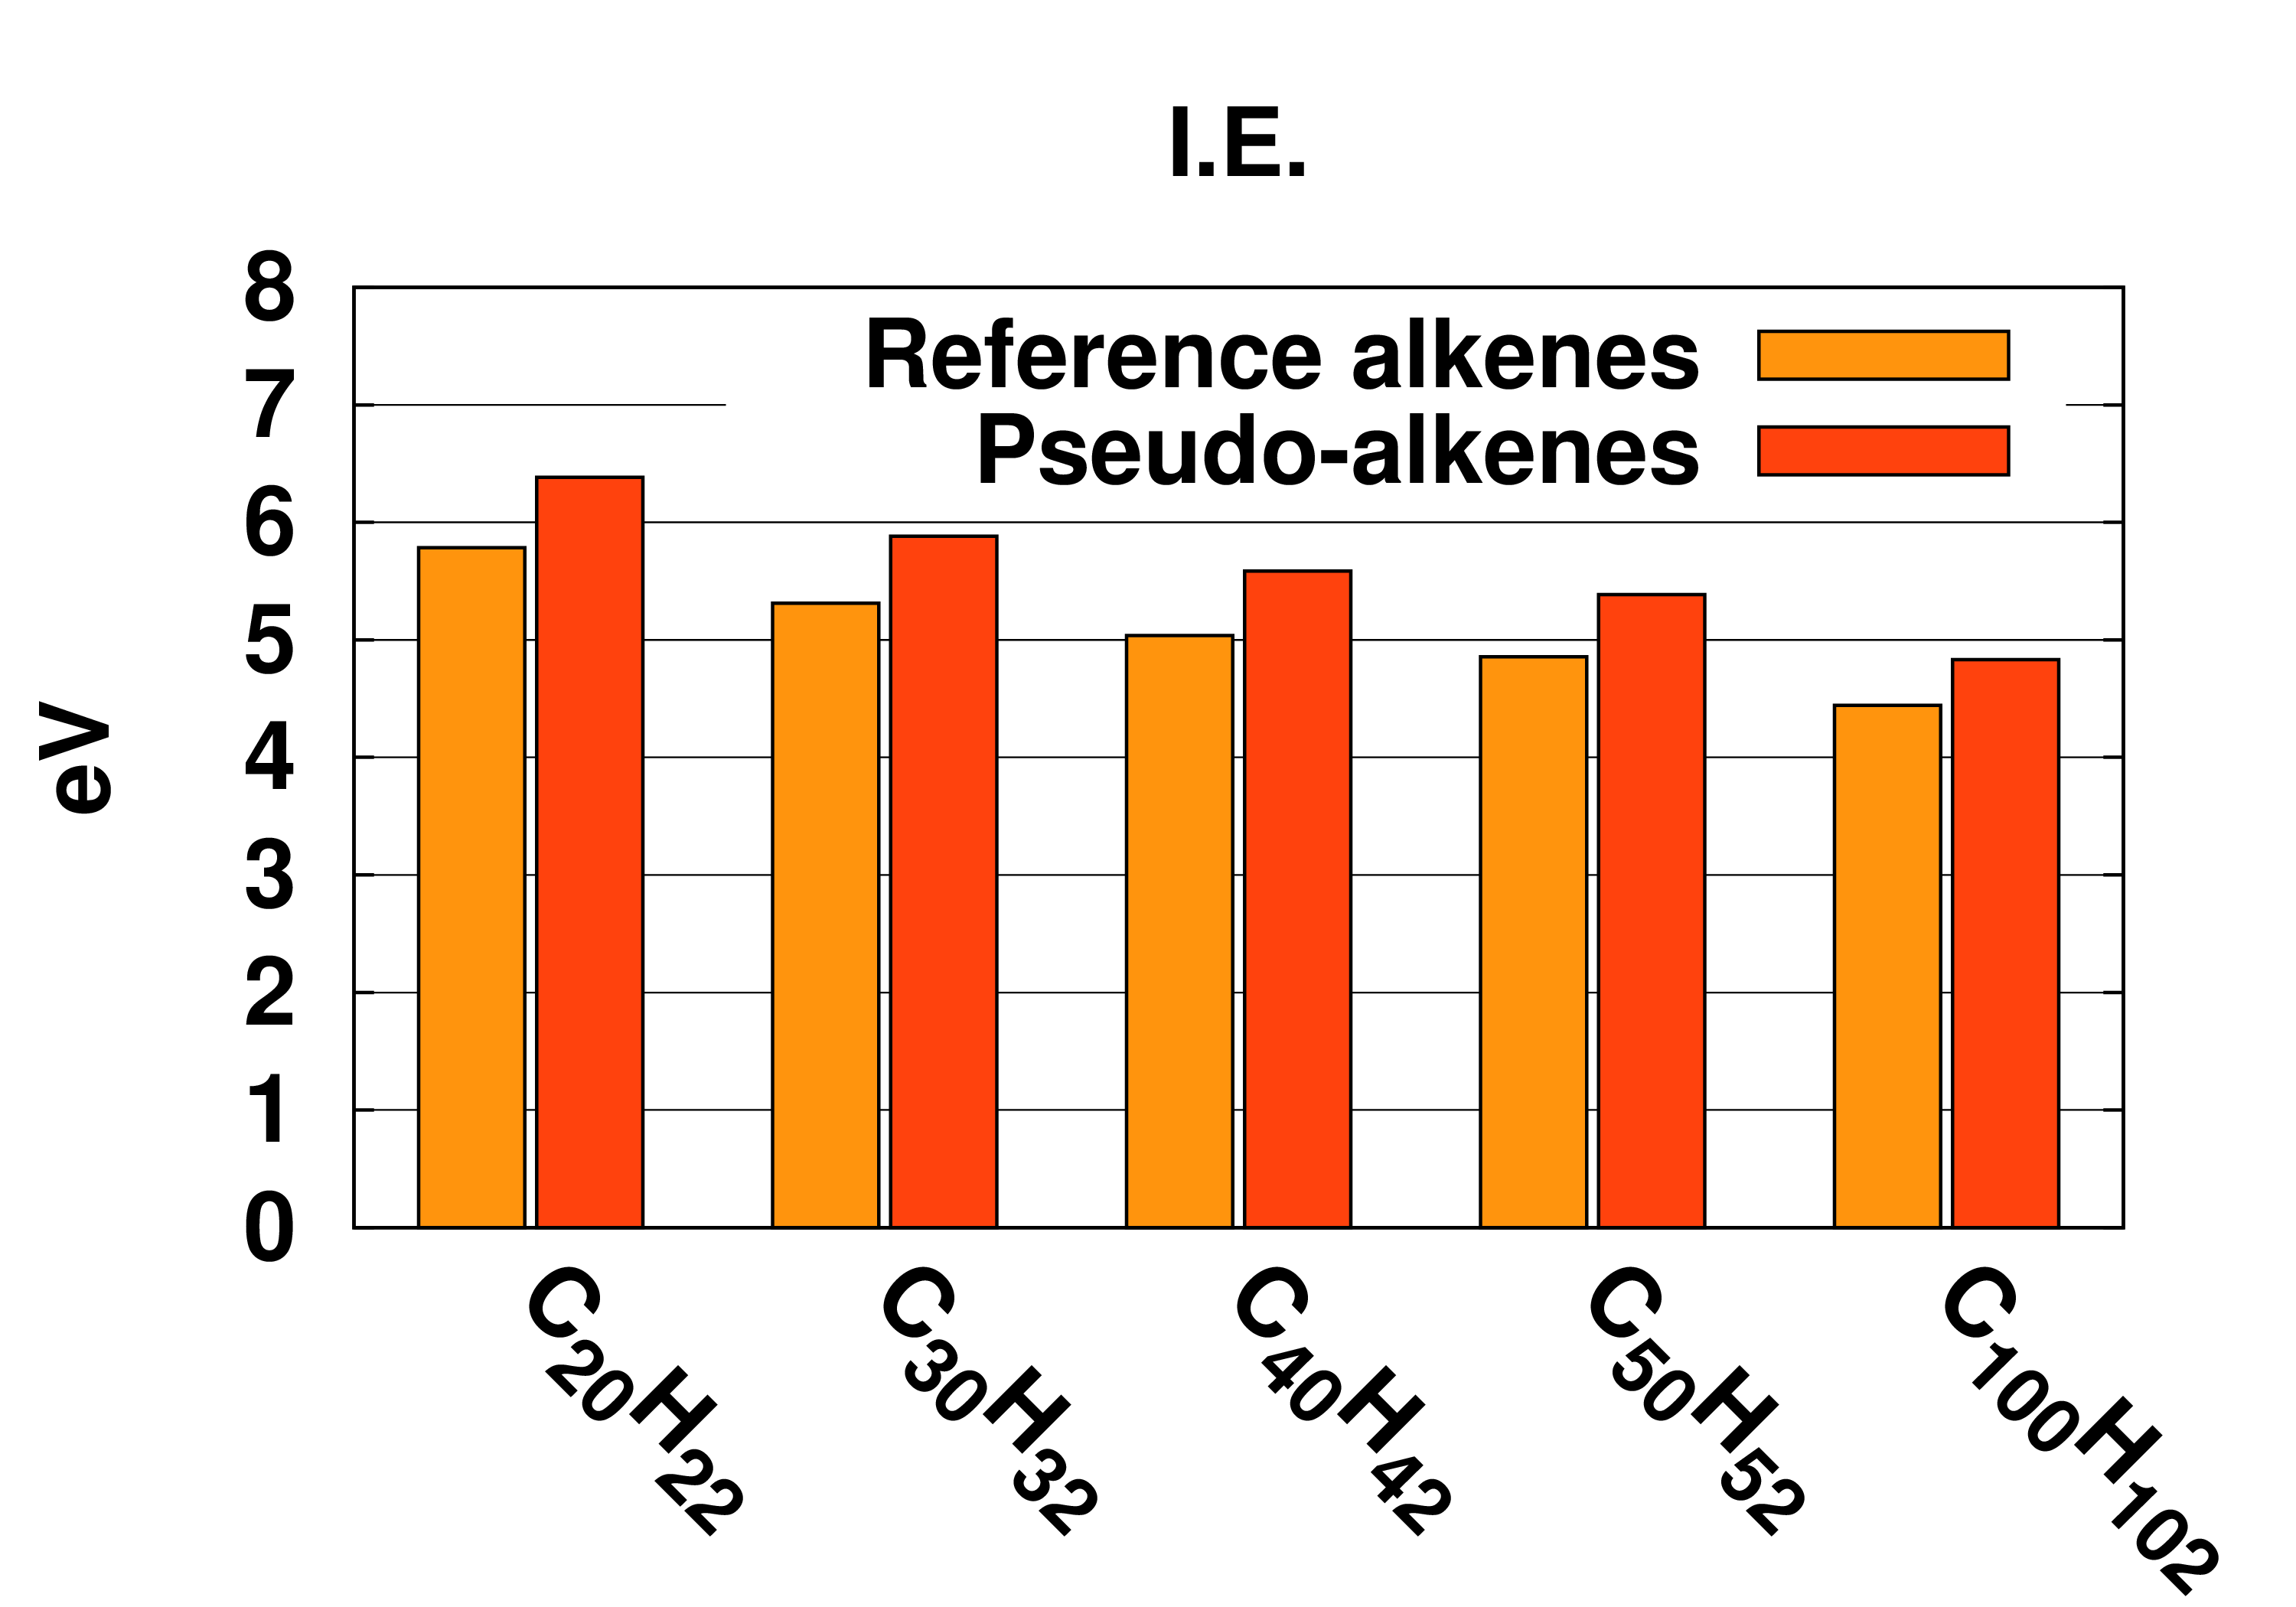
\includegraphics[width=8cm]{long_pbe0_ie}
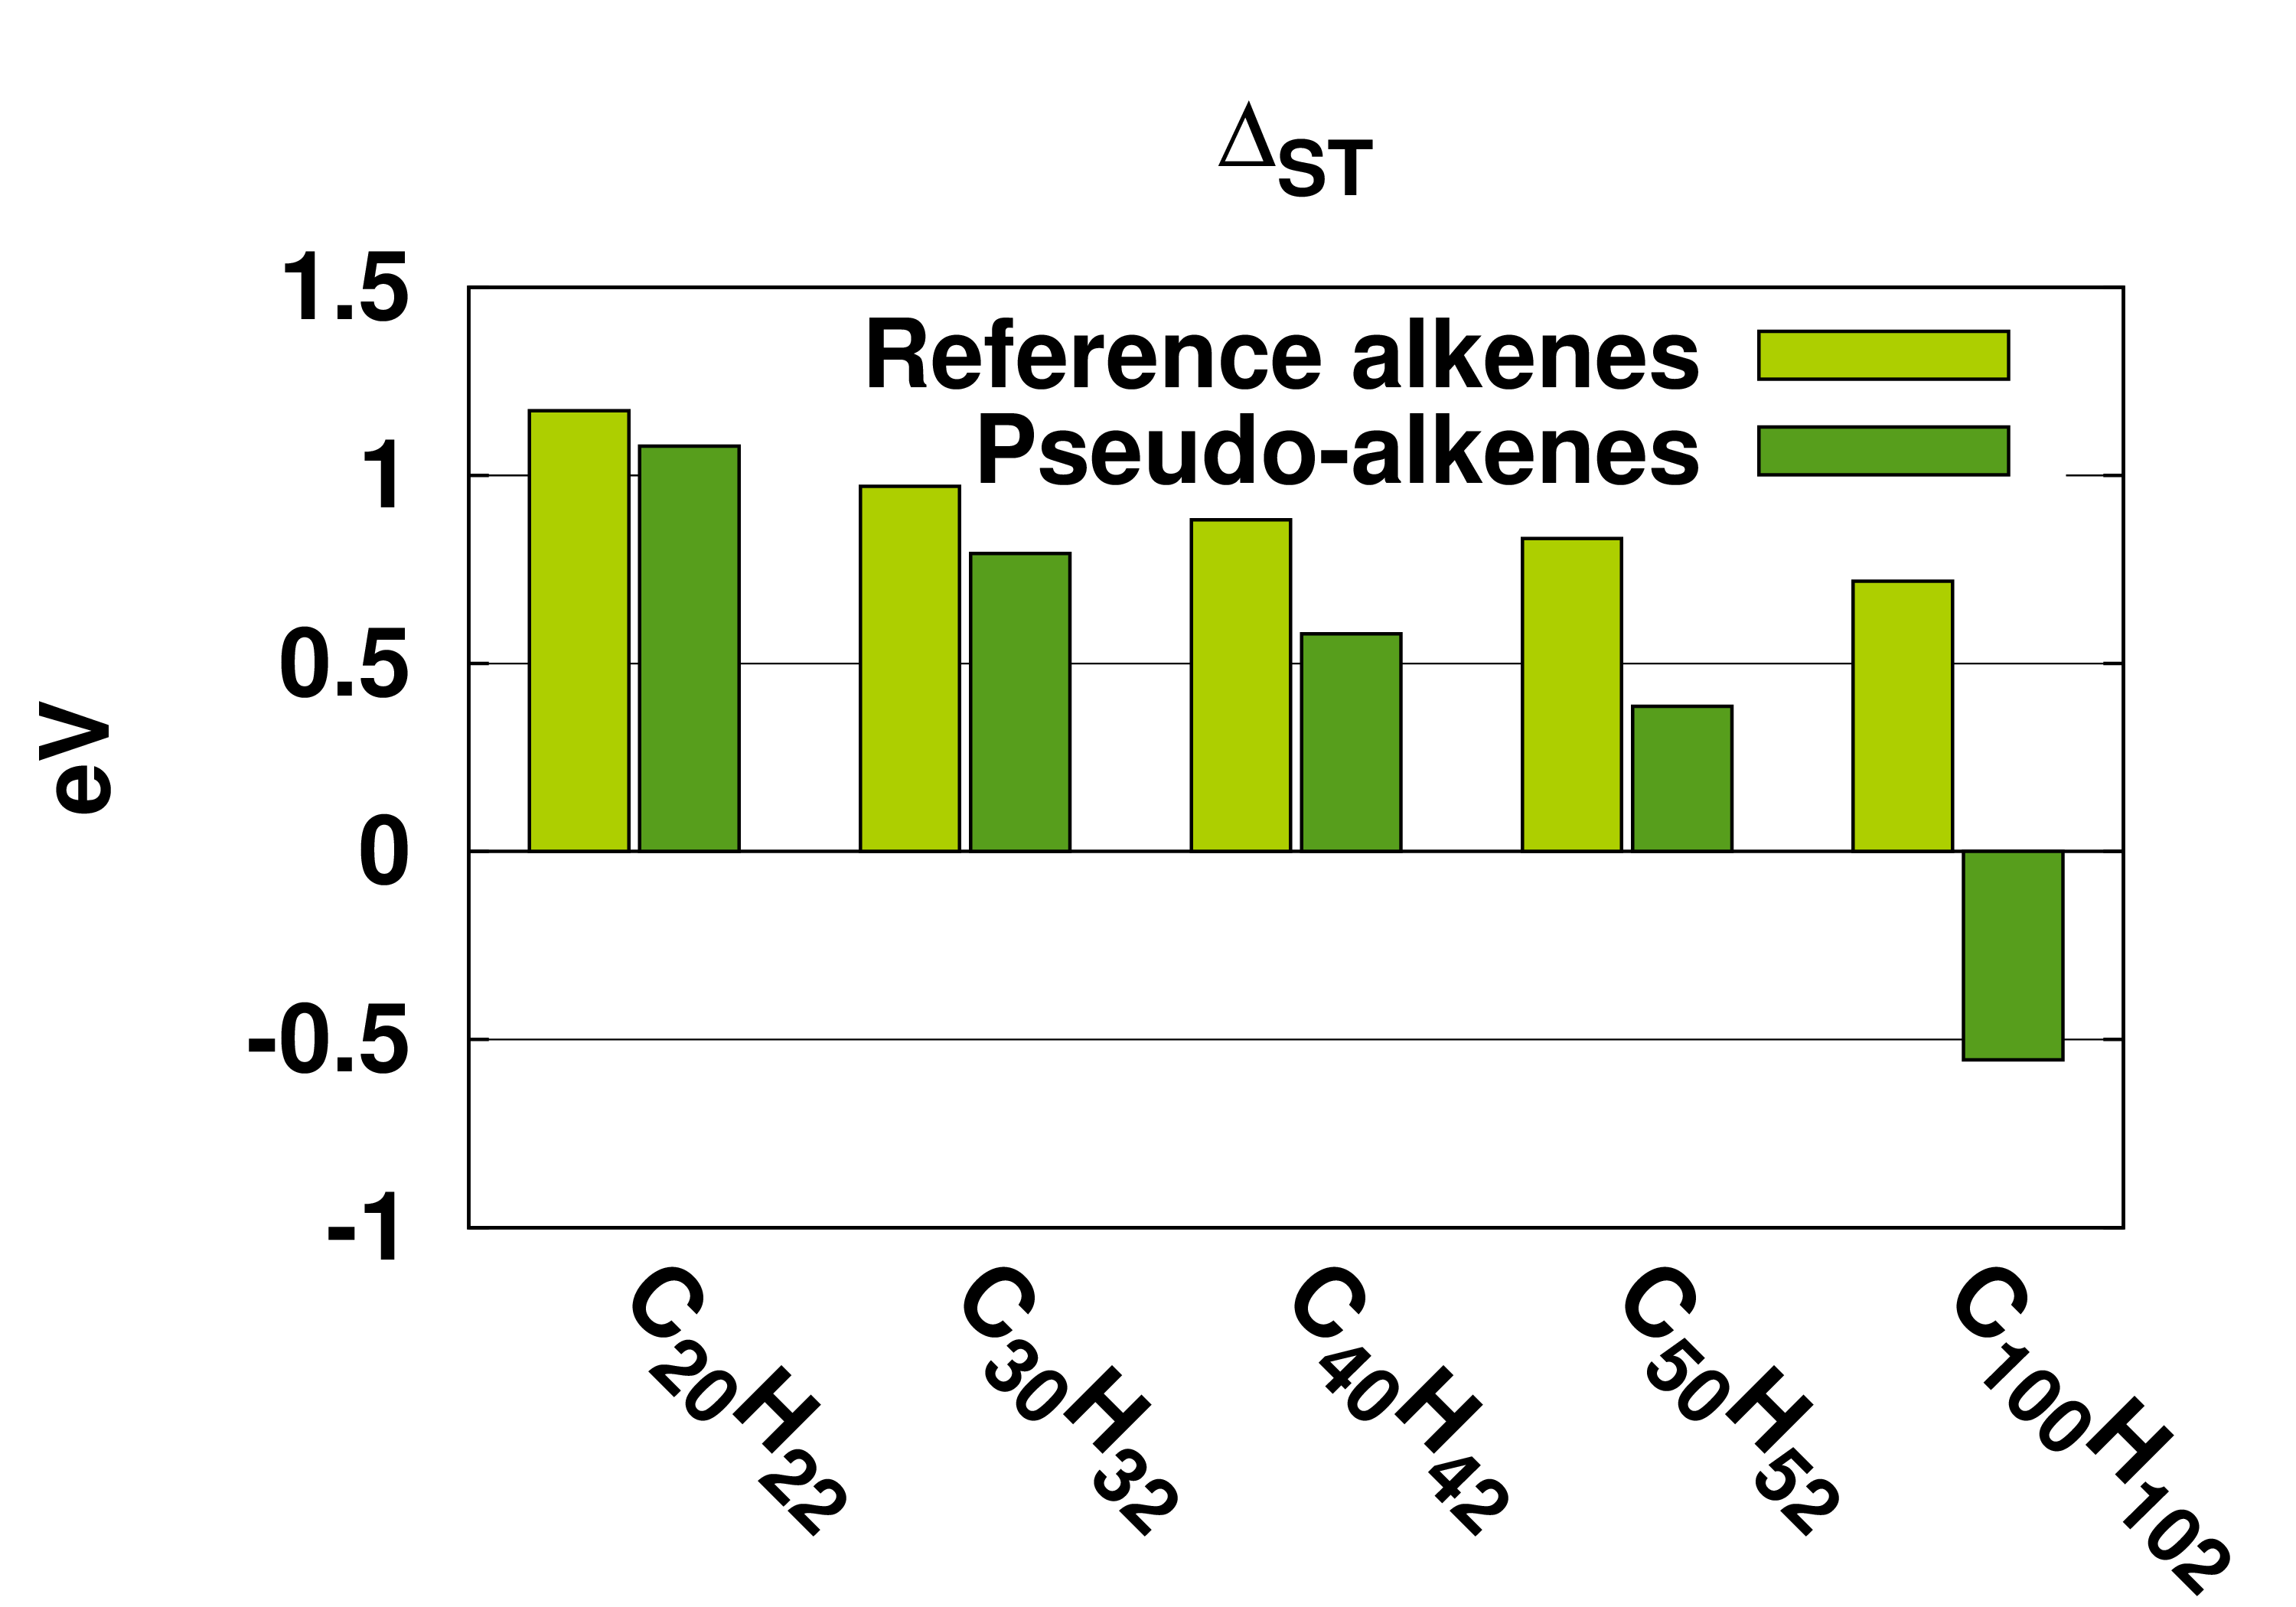
\includegraphics[width=8cm]{long_pbe0_st}
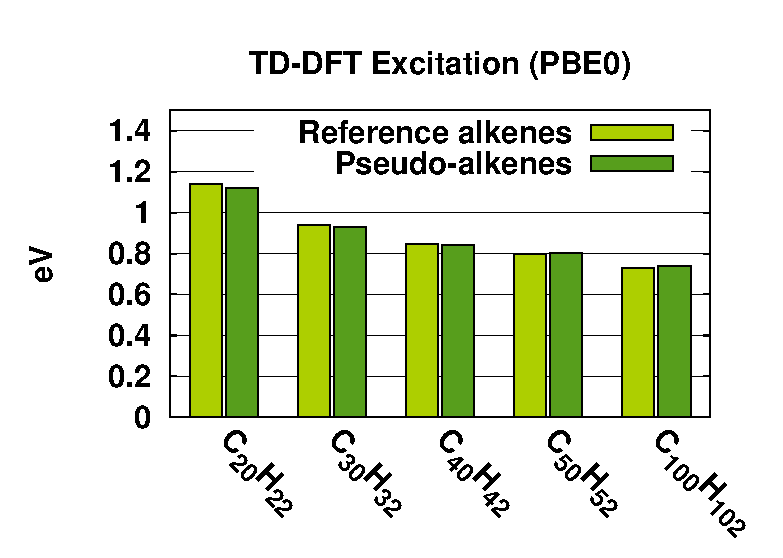
\includegraphics[width=8cm]{long_pbe0_tddft}
\end{center}

\caption{Comparison of the HOMO energy ($\varepsilon_{HOMO}$),
the ionisation energy (I.E.),
the first singlet-triplet excitation energy ($\Delta_{ST}$) and
the TD-DFT first excitation energy
between the
all electron reference system and the optimal pseudo-potential across a range of long chain alkenes (C\(_{20}\)-C\(_{100}\)).
The $\Delta_{ST}$ values were obtained as the difference
between the lowest triplet (in an unrestricted formalism) and the lowest singlet state
(in a restricted formalism).
Calculations were done at the PBE0/def-SV(P) level.}
\label{fig:long_chain_graphs}
\end{figure}

\begin{table}[ht]
\begin{tabular}{l r r r r r }
\hline\hline
                 & HF & PBE0 & PBE & TPSS & TPSSH \\
\hline
$\varepsilon_{HOMO}$    &  1.8 &  7.3   &  11.3   &  16.7    &  13.6 \\
I.E.                    & 25.1 &  6.7   &   9.4   &  10.3    &  11.6 \\
$\Delta_{ST}$           & 55.3 & 85.8   &  83.4   & 239.8    & 320.2 \\
TD-DFT First Excitation &    - &  0.005 &   0.043 &    0.033 &   0.001 \\ 
\hline\hline
\end{tabular}
\caption{Mean relative errors (in percent) across methods (HF or different functionals)
for long chain alkenes (C\(_{20}\)-C\(_{100}\)).}
\label{table:long_alkene_errors}
\end{table}

The pattern of decreasing ionisation potentials and $\Delta_{ST}$ with increasing HOMO
energy is still followed, with the absolute error remaining consistent.
However, differences in the triplet-singlet energies between the reference and pseudo-systems 
become significant, notably for the largest case.

Unlike for the previous systems, there is a large discrepancy between $\Delta_{ST}$
and TD-DFT results.
This apparent failure of the pseudo-potentials is to be found in the representation
of the triplet state. The expectation values of the $S^2$ operator for the triplet calculations
are plotted in Figure \ref{fig:ssquare}, which shows that the spin contamination
of the triplet state computed as a single configuration (\emph{i.e.} in a SCF
framework) increases in both reference and pseudo-potential cases.
Yet, this effect is strengthened in the pseudo-potential calculations.
These results suggest that the triplet state cannot be represented as one configuration
but as a linear combination of mono-electronic excitations as done through TD-DFT.

\begin{figure}
\begin{center}
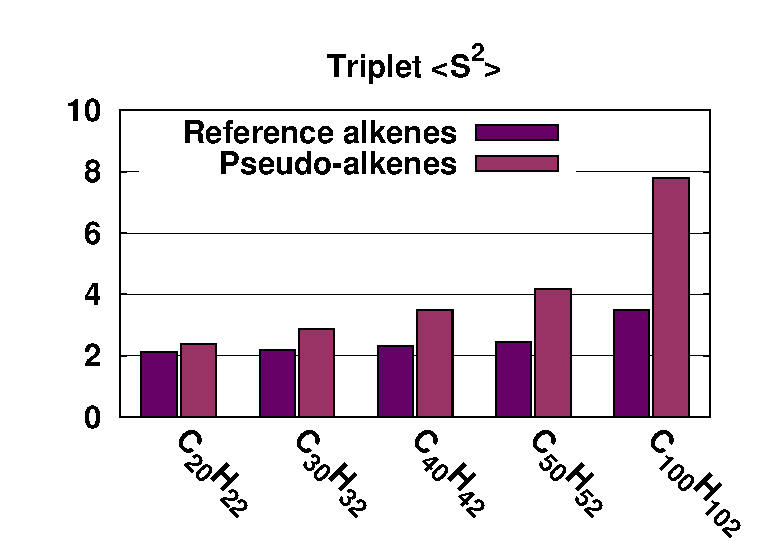
\includegraphics[width=8cm]{long_pbe0_s2}
%\caption{Comparison of $S^2$ expectation values obtained for the calculation
%of the first triplet configuration in a SCF formalism, for reference
%and pseudo-systems.}
%\label{fig:ssquare}
\end{center}
\caption{Comparison of $S^2$ expectation values obtained for the calculation
of the first triplet configuration in a SCF formalism, for reference
and pseudo-systems.}
\label{fig:ssquare}
\end{figure}

\begin{table}[ht]
\begin{tabular}{c c r r}
\hline\hline
\multicolumn{2}{c}{Excitation} & \multicolumn{2}{c}{Weight(\%)}\\
\multicolumn{2}{c}{MO} & Ref. & Pseudo.\\
\hline
\multicolumn{2}{c}{25 a" \(\rightarrow\) 26 a"} & 77.0 &   67.1  \\
\multicolumn{2}{c}{24 a" \(\rightarrow\) 27 a"} & 10.5 &   13.1  \\
\multicolumn{2}{c}{23 a" \(\rightarrow\) 28 a"} & 3.6  &    5.2  \\
\hline\hline
\end{tabular}
\caption{\label{tab:coef}Comparison of the weights (all electron \emph{vs.} pseudo-potentials)
of the excitations obtained with TD-DFT
to represent the triplet excited state from the closed shell singlet state.
Example case of C$_{50}$H$_{52}$.}
\end{table}

In order to show that the recovering of the agreement between the pseudo-potential
and the reference calculations is not an artefact, we give in Table~\ref{tab:coef}
the weight and nature of each excitation (weight larger than 3\%)
in the description of the triplet excited state for
C$_{50}$H$_{52}$ (other values can be found in the SI, which exhibit the same trends).
As can be seen, the agreement is very good. 

These results show that the pseudo-potentials that we have extracted are able to reproduce the
$\pi$ systems in a variety of situations which are not part of their extraction set.
The molecular orbital virtual space is also well described (cf. Table~\ref{tab:coef}),
which demonstrates that the good agreement with reference calculations is
physically grounded.

\clearpage

\section{Conclusion}
In this work, we tackled the two main problems of the initial version of our
molecular potentials.
Firstly, the new pseudo-potentials for sp$^2$ hybridised
atoms are completely atomic and, even if the directionality of the bonding pattern
has to be fullfilled by correctly positioning the \(s\) potentials, no potentials need to
be added relative to the position of two atoms.
Secondly, we gave a physical meaning to all the pseudo-potential
terms.
Contrary to our previous attempt, we do not rely on the "no collapse" term,
which is modeled here by forcing the molecular occupation (\emph{vide infra}).
We could show that not only were the occupied orbitals well-reproduced
by the use of these new potentials, but also that the virtual space is of good quality
for excited states calculation.

In the framework of this study, there are three logical next steps: the addition of an explicit
"no collapse" term, the reproduction of the gradient through the parameterisation
of additional terms, and finally the use of such potentials in the framework
of QM/MM calculations as a replacement of hydrogen based link atoms.
The first step is needed in order to avoid forcing the molecular orbital occupation and
to avoid spurious virtual orbitals in the active space.
We are confident that the first step could be easily done, as we have already extracted such
terms in the previous version of our potentials.
The reproduction of the gradient is more of a challenge as many electrons were removed from the system.
Finally, QM/MM tests can be started quickly, as we could fix the local geometry of the potentials
in the QM part. The MM part would be taken care of without modification of the standard parameters.

%%%%%%%%%%%%%%%%%%%%%%%%%%%%%%%%%%%%%%%%%%%%%%%%%%%%%%%%%%%%%%%%%%%%%%%%%%%%%%%%%
% BIBLIOGRAPHY

\bibliography{biblio_pseudo_alex}   % Produces the bibliography via BibTeX.

%\begin{thebibliography}{99}
%
%
%\bibitem{Coulson}
%Coulson, C. A., Rev. Mod. Phys., \textbf{1960}, 32,170-177.
%\bibitem{Malrieu}
%Malrieu, J.-P., J. Mol. Struct., \textbf{1998}, 424, 1-2,83-91.
%\bibitem{Shaik}
%Shaik, S., New. J. Chem., \textbf{2007}, 31,2015-2028.
%\bibitem{Hoffmann}
%Hoffman, R., Schleyer, P. v. R., Schaefer III, H. F., \textbf{2008}, 47, 7164-7167.
%\bibitem{Perdew}
%Perdew, J. P., Ruzsinszky, A., Constantin, L., Sun, J., Csonka, G., J. Chem. Theory Comput., \textbf{2009}, 5, 902-908.
%\bibitem{Koros}
%Koros, W. J.; Chern, R. T. In Handbook of Separation Process Technology; Rousseau, E. D.; Russell, B., Eds.; Wiley: New York, \textbf{1987}; Vol. 2, Chapter 20, pp 34-45.
%\end{thebibliography}


%%%%%%%%%%%%%%%%%%%%%%%%%%%%%%%%%%%%%%%%%%%%%%%%%%%%%%%%%%%%%%%%%%%%%%%%%%%%%%%%%

\clearpage
\section{Supplementary materials}
\subsection{Details on the extraction process}
\subsubsection{CH\(_{3}\), with \(s\)-potentials}

We aim first at reproducing the values for the CH\(^{\bullet}_{3}\) radical as given in Table \ref{table:ch3_s_potentials}. 
This reference CH\(^{\bullet}_{3}\) is created and has its geometry optimised under Hartree-Fock (HF). The reference geometry gives a C - H distance of 2.0466 a.u., and so we pick \(d = 2.0\) a.u. as a starting guess for the planar distance from the pseudo-carbon, \(d\), of our pseudo-potentials. The pseudo-system is then set up, erasing the hydrogen atoms, setting the carbon charge \(Z_{nucleus} = 1\) and applying \(s\) pseudo-potentials, as well as selecting the correct orbital for the remaining electron. Table \ref{table:ch3_s_potentials} displays some of our results. Promisingly, we are able to produce many sets of potentials that give the correct energy.

\subsubsection{Ethene, with \(s\) and \(p\)-potentials}

Next, we take some of these potentials to create a pseudo-ethene system, with the results shown in Table \ref{table:ethene_s_pseudo}. All potentials tested with \(d = 2.0\) a.u. gave results several orders of magnitude away from the reference value. From Figure \ref{fig:long_r_ethene} we may see the reason. One of the potential sets from each carbon is closer to the neighbouring carbon than the neighbour's own potential sets, thus both pseudo-carbons are affected by potentials which do not belong to them. At the shorter range \(d = 0.5\) a.u., the HOMO energy is of the right magnitude, though with errors of \(~ 30\%\). Attempts to eliminate this error lead us to the additional use of the \(p_{z}\) potential \textit{alongside} the \(s\) potentials.

The next step adds a \(p\)-potential centred on the pseudo-carbon, with Table \ref{table:p_potentials} displaying the results. As before, \(d = 0.5\) a.u.. The \(p_{z}\) potential is selected using the procedure described in Section \ref{section:potential_derivation}, with the exponent chosen to give the maximum possible overlap with the \(p_{z}\) orbital, and the matching \(Z_{eff}\) coefficient calculated from the exponent and overlap. The \(s\)-potentials are then optimised once more to give the correct HOMO energy for CH\(^{\bullet}_{3}\). We again take these potentials to create a pseudo-ethene molecule, with the results shown in Table \ref{table:p_potentials}. We can see that these potentials seem to transfer more effectively from the CH\(^{\bullet}_{3}\) system to the ethene, suggesting therefore that whilst the \(s\)-potentials can affect both the \(p_{z}\) and \(\pi\) orbitals, they 
cannot alone describe the relationship between them.

Having successfully created a pseudo-ethene with the correct HOMO, we attempt to have the pseudo-system replicate other properties of the real system:
the singlet-triplet excitation energy ($\Delta_{ST}$) in the SCF framework (energy difference between the triplet and the singlet mono-reference
calculations), the ionisation energy (IE) and the energy of the HOMO orbital ($\varepsilon_{HOMO}$). Reference values for the singlet-triplet \(\pi-\pi*\) excitation and first ionisation energies of ethene are given in Table \ref{table:ethene_excitations}. Testing the relevant energies for the optimised pseudo-systems above, we can see from Table \ref{table:ethene_excitations} that the early results are not promising. However, after we abandon the notion of sticking strictly to a \(p_{z}\)-potential exponent that gives the maximum overlap with the real orbital, we discover there is a "sweet spot" of potential coefficients and exponents around which the correct values begin to emerge. Table \ref{table:ethene_excitations} shows our optimal result, chosen to give HOMO, triplet - singlet and ionisation energies closest to the reference values. 

\subsubsection{Optimisation}

In earlier calculations with only \(s\)-potentials, optimisation was performed by choosing a range of exponent values and attempting to optimise the coefficient at each to produce the HOMO reference energy. Once the \(p_{z}\) potential was added, the \(s\)-potentials were optimised afterward. 

Once we started to look at excitation and ionisation energies however, optimisation became more complicated. Optimisations were at first performed of the s and p-potentials to reach the HOMO energy of ethene as before. With the different potential variables available, we produced a range of optimised potential sets. The best set of these potentials was then chosen and the values altered by hand in order to match as closely as possible three separate reference values: the singlet HOMO energy, the singlet-triplet \(\pi-\pi*\) excitation energy, and the cation-singlet energy. All optimisations used the Brent method in SciPy's optimisation library, with a tolerance of \(1.48*10^{-08}\), and used standard Hartree-Fock calculations.\cite{scipy}

\subsection{Comparison with our previous study}
\begin{figure}
\begin{center}
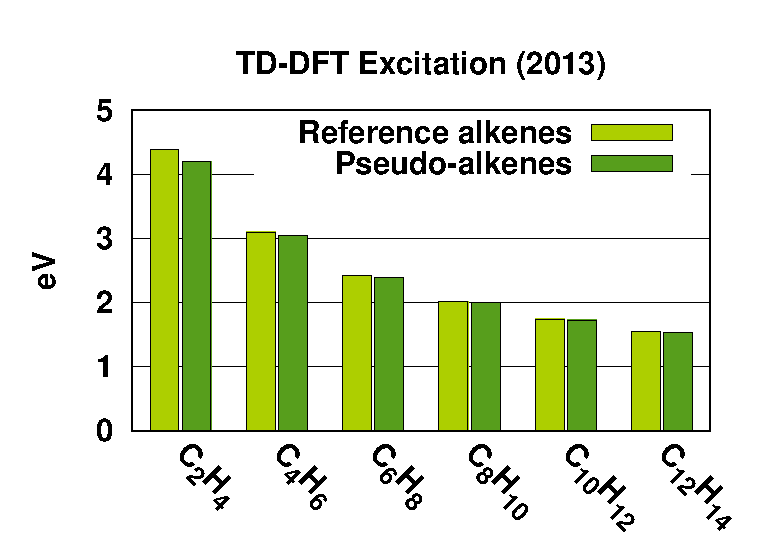
\includegraphics[width=8cm]{short_pbe0_tddft_2013}
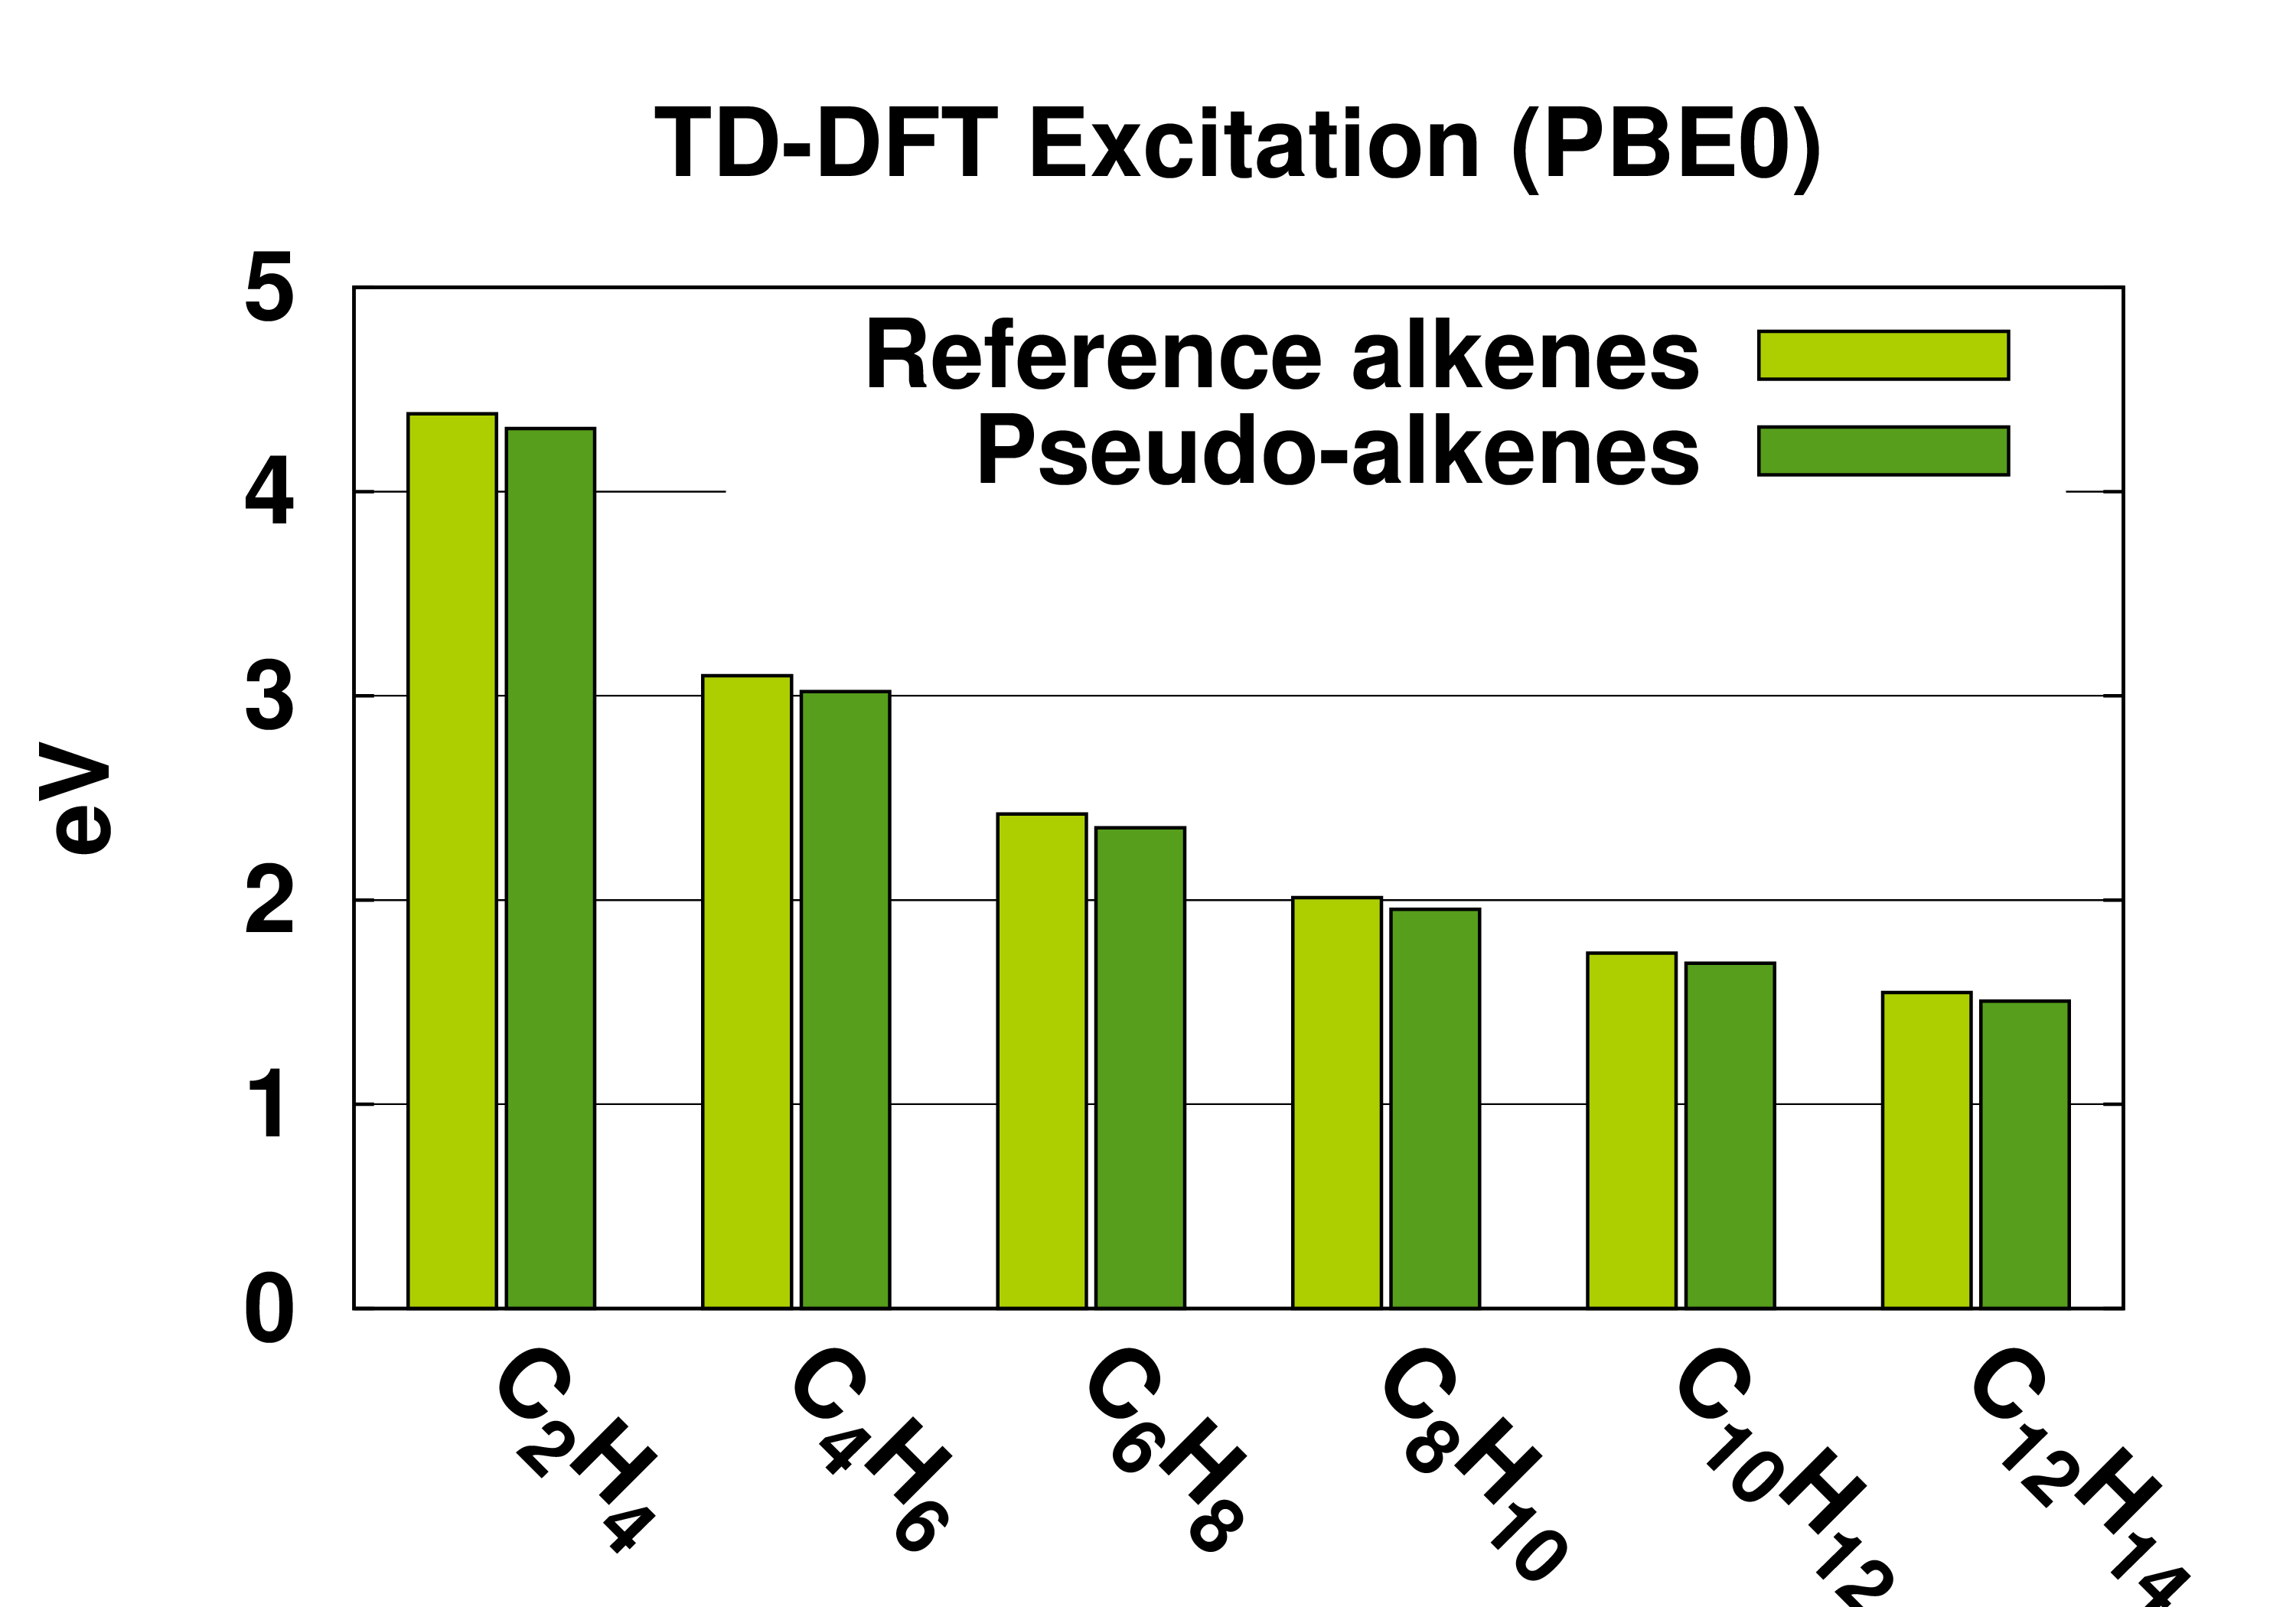
\includegraphics[width=8cm]{short_pbe0_tddft}
\end{center}
\caption{Comparison of pseudo-alkenes with previous\cite{drujon_pseudopotentials_2013} and current potentials using TD-DFT excitation energies.}
\label{fig:alkenes_tddft}
\end{figure}

%%%%%%%%%%%%%%%%%%%%%%%%%%%%%%%%%%%%%%%%%%%%%%%%%%%%%%%%%%%%%%%%%%%%%%%%%%%%%%%%%
% FIGURE CAPTIONS

%%%%% FIGURE ---- cc.eps
\begin{figure}
\begin{center}
%\includegraphics[width=0.2\columnwidth,keepaspectratio=true]{cc.eps}
\fbox{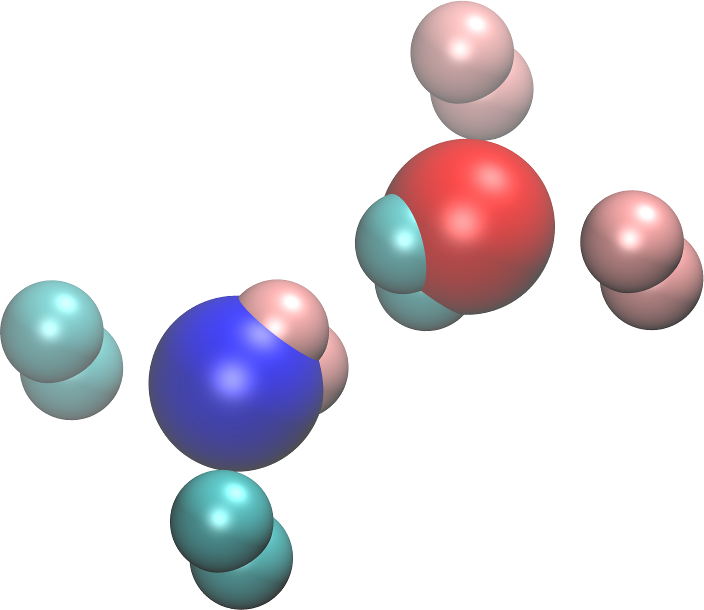
\includegraphics[width=0.45\textwidth]{hires_long_r_crop.png}}%
\fbox{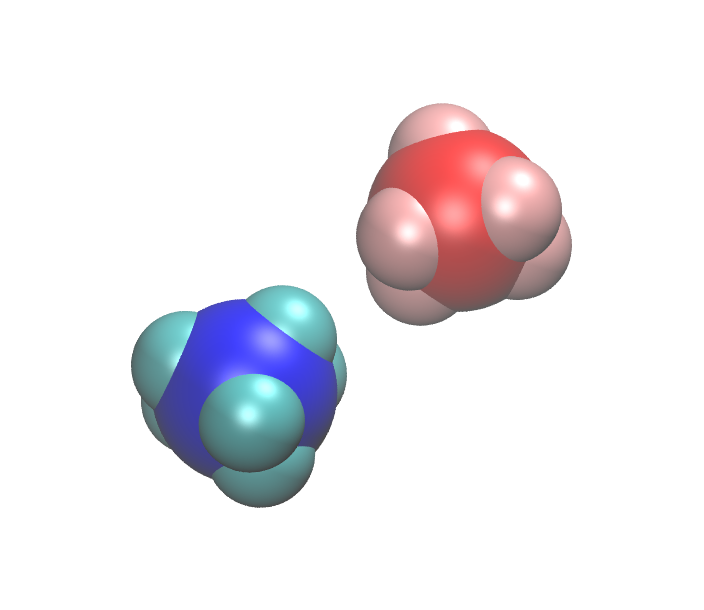
\includegraphics[width=0.45\textwidth]{hires_short_r_crop.png}}
\end{center}
\caption{Diagrams of pseudo-ethene with \(d =\) 2.0 a.u. (left), and \(d = 0.5\) a.u. (right). The first pseudo-carbon is displayed in blue, with its \(s\) pseudo-potentials in cyan, and the second pseudo-carbon is in red, with its potentials in pink.}
\label{fig:long_r_ethene}
\end{figure}
%%%%%%%%%%%%%%%%%%%%%%%%%%%%
\clearpage

\begin{table}[ht]
\begin{tabular}{c c c}
\hline\hline
 & Coefficient & Exponent \\ 
\hline
HF & -2.594 & 1.0 \\
 & -4.788 & 5.0 \\
 & -7.524 & 10.0 \\
\hline
PBE0 & -2.605 & 1.0 \\
 & -4.873 & 5.0 \\
 & -7.678 & 10.0 \\
\hline\hline
\end{tabular}
\caption{Coefficients and exponents for \(s\)-only pseudo-potentials for CH\(^{\bullet}_{3}\), optimised to give 
the all-electron HOMO reference energy of  -10.537~eV (HF) and -6.726~eV (PBE0). 
\(d = 0.5\) a.u., as defined in Figure~\ref{figure:ref_pseudo_diagram}.}
\label{table:ch3_s_potentials}
\end{table}

\newpage

\begin{table}[ht]
\begin{tabular}{c c c c}
\hline\hline
& $d$ & \(s\) coefficient & \( \pi \)  \\
\hline
HF$^a$   &     &        & -10.363 \\
PBE0$^a$ &     &        & -6.632 \\
HF       & 2.0 & -7.521 & -9597.0 \\
HF       & 0.5 & -7.521  & -7.905 \\
PBE0     & 0.5 &-7.678  & -8.447 \\
\hline\hline
\multicolumn{4}{l}{$^a$ All-electron reference values.}\\
\end{tabular}
\caption{HOMO energies ($\pi$, eV) for ethene and pseudo-ethene. The pseudo-potentials used in the pseudo-ethene are taken from optimised values for 
pseudo-CH\(^{\bullet}_{3}\) with only \(s\)-potentials and an exponent of 10.0. $d$ (a.u.) as defined 
in Figure~\ref{figure:ref_pseudo_diagram}.}
\label{table:ethene_s_pseudo}
\end{table}

\newpage

\begin{table}[ht]
\begin{tabular}{c c c c}
\hline\hline
& \(p\) coefficient & \(p\) exponent \\
\hline
\(p_{z}\) potential & -3.267 & 0.295 \\
\hline
Calculation Type & \(s\) coefficient & \(s\) exponent & \(\pi\) \\
\hline
HF & 2.772 & 1.0 & -13.654 \\
 & 6.173 & 5.0 & -14.011 \\
 & 10.381 & 10.0 & -14.061 \\
\hline
PBE0 & 3.483 & 1.0 & -10.325 \\
 & 9.801 & 5.0 & -10.409 \\
 & 18.351 & 10.0 & -12.543 \\
\hline\hline
\end{tabular}
\caption{\(\pi\) orbital energy values (eV) for pseudo-ethene, using \(s\) and \(p\) pseudo-potentials.
The pseudo-potentials are taken from a pseudo-CH\(^{\bullet}_{3}\) system optimised to give the correct all-electron HOMO energy.}
\label{table:p_potentials}
\end{table}

%\subsection{Geometry Optimisation}
%\label{section:geometry_optimisation}
%
%Using pseudo-potential calculations for geometry optimisation presents some difficulties. Designing pseudo-potentials such that the explicitly-treated parts of the molecule experience the correct attraction and repulsion at a particular geometry is one thing, designing them such that the same is true at any (reasonable) geometry is quite another. With a little knowledge of the all-electron system however, we can ensure that the pseudo-system will fall into the correct geometry.
%
%We begin by finding curves of dissociation for the explicit and pseudo-potential parts of the molecule, as well as another for the same parts of the all-electron molecule (see Fig \ref{fig:dissociation_diagram}). We then use a nonlinear least-squares Marquardt-Levenburg algorithm to fit a simple, exponentially-decreasing function to the difference between thsese two curves. We can now use this to make an energy correction to the pseudo-system. 
% 
%We want the total energy of the system to be a minimum and the energy gradients on the explicitly-treated atoms to be zero at the true geometry (this needn't be true of the pseudo-atoms, see below). We have the correction for the total energy, and by taking the derivative of the fitted function, we have a measure of whether the explicit and pseudo-potential parts of the molecule experience an overall attraction or repulsion, as well as an estimate of its magnitude. We assume the effect of the potentials on the explicit hydrogen atoms is small, and add our gradient correction directly to the potential felt along the carbon-pseudo-carbon axis by one carbon, whilst subtracting it from the potential felt by the other. By doing this at every step of the optimisation, the carbon-pseudo-carbon distance should naturally reach the correct value.
%
%Finally, the pseudo-atoms are fixed relative to each other before starting the optimisation.
%
%\begin{figure}
%\begin{center}
%\end{center}
%\caption{Diagram of dissociation curves for all-electron and pseudo-molecular calculations.}
%\label{figure:dissociation_diagram}
%\end{figure}

\end{document}

